\documentclass{article}
\usepackage{geometry}
\usepackage{graphicx}
\usepackage{float}
\usepackage{titlesec}
\geometry{a4paper, left=2cm, right=2cm, top=2cm, bottom=2cm}
\titleformat{\section}{\normalfont\fontsize{14}{15}\bfseries}{\thesection}{1em}{}
\usepackage{hyperref}
\usepackage{graphicx}
\usepackage{ctex}
\usepackage{caption}
\usepackage{subcaption}
\usepackage{listings}
\usepackage{xcolor}

% 设置代码样式
\lstdefinestyle{Style}{
    language=Scala, % 设置代码语言
    basicstyle=\ttfamily\small, % 设置字体样式和大小
    keywordstyle=\color{blue}, % 关键字颜色
    commentstyle=\color{green!40!black}, % 注释颜色
    stringstyle=\color{purple}, % 字符串颜色
    numbers=left, % 行号显示在左侧
    numberstyle=\tiny\color{gray}, % 行号样式
    stepnumber=1, % 行号逐行显示
    numbersep=8pt, % 行号与代码的距离
    showspaces=false, % 是否显示空格
    showstringspaces=false, % 是否显示字符串中的空格
    showtabs=false, % 是否显示制表符
    tabsize=4, % 制表符的大小
    frame=single, % 边框类型,可以是 single, lines, none, ...
    frameround=tttt, % 边框角落样式,可以是 tttt, trbl, none, ...
    backgroundcolor=\color{white}, % 背景颜色
    breaklines=true, % 自动断行
    breakatwhitespace=true, % 在空格处断行
    captionpos=b, % 代码块标题位置(b 表示底部)
    extendedchars=true, % 支持特殊字符
    morekeywords={val, var, def, import}, % 添加额外的关键字
    inputencoding=utf8, % 输入编码,适用于包含非 ASCII 字符的代码
}

\begin{document}
\title{大数据分析云平台环境配置与测试}
\author{211250109 赵政杰}
\date{\today}
\maketitle

\section{环境配置}

\subsection*{1.1 选择平台并创建实例}
在此我选用阿里云,它为学生提供一个月的免费服务器。创建实例后通过控制台查看。
\begin{figure}[H]
    \centering
    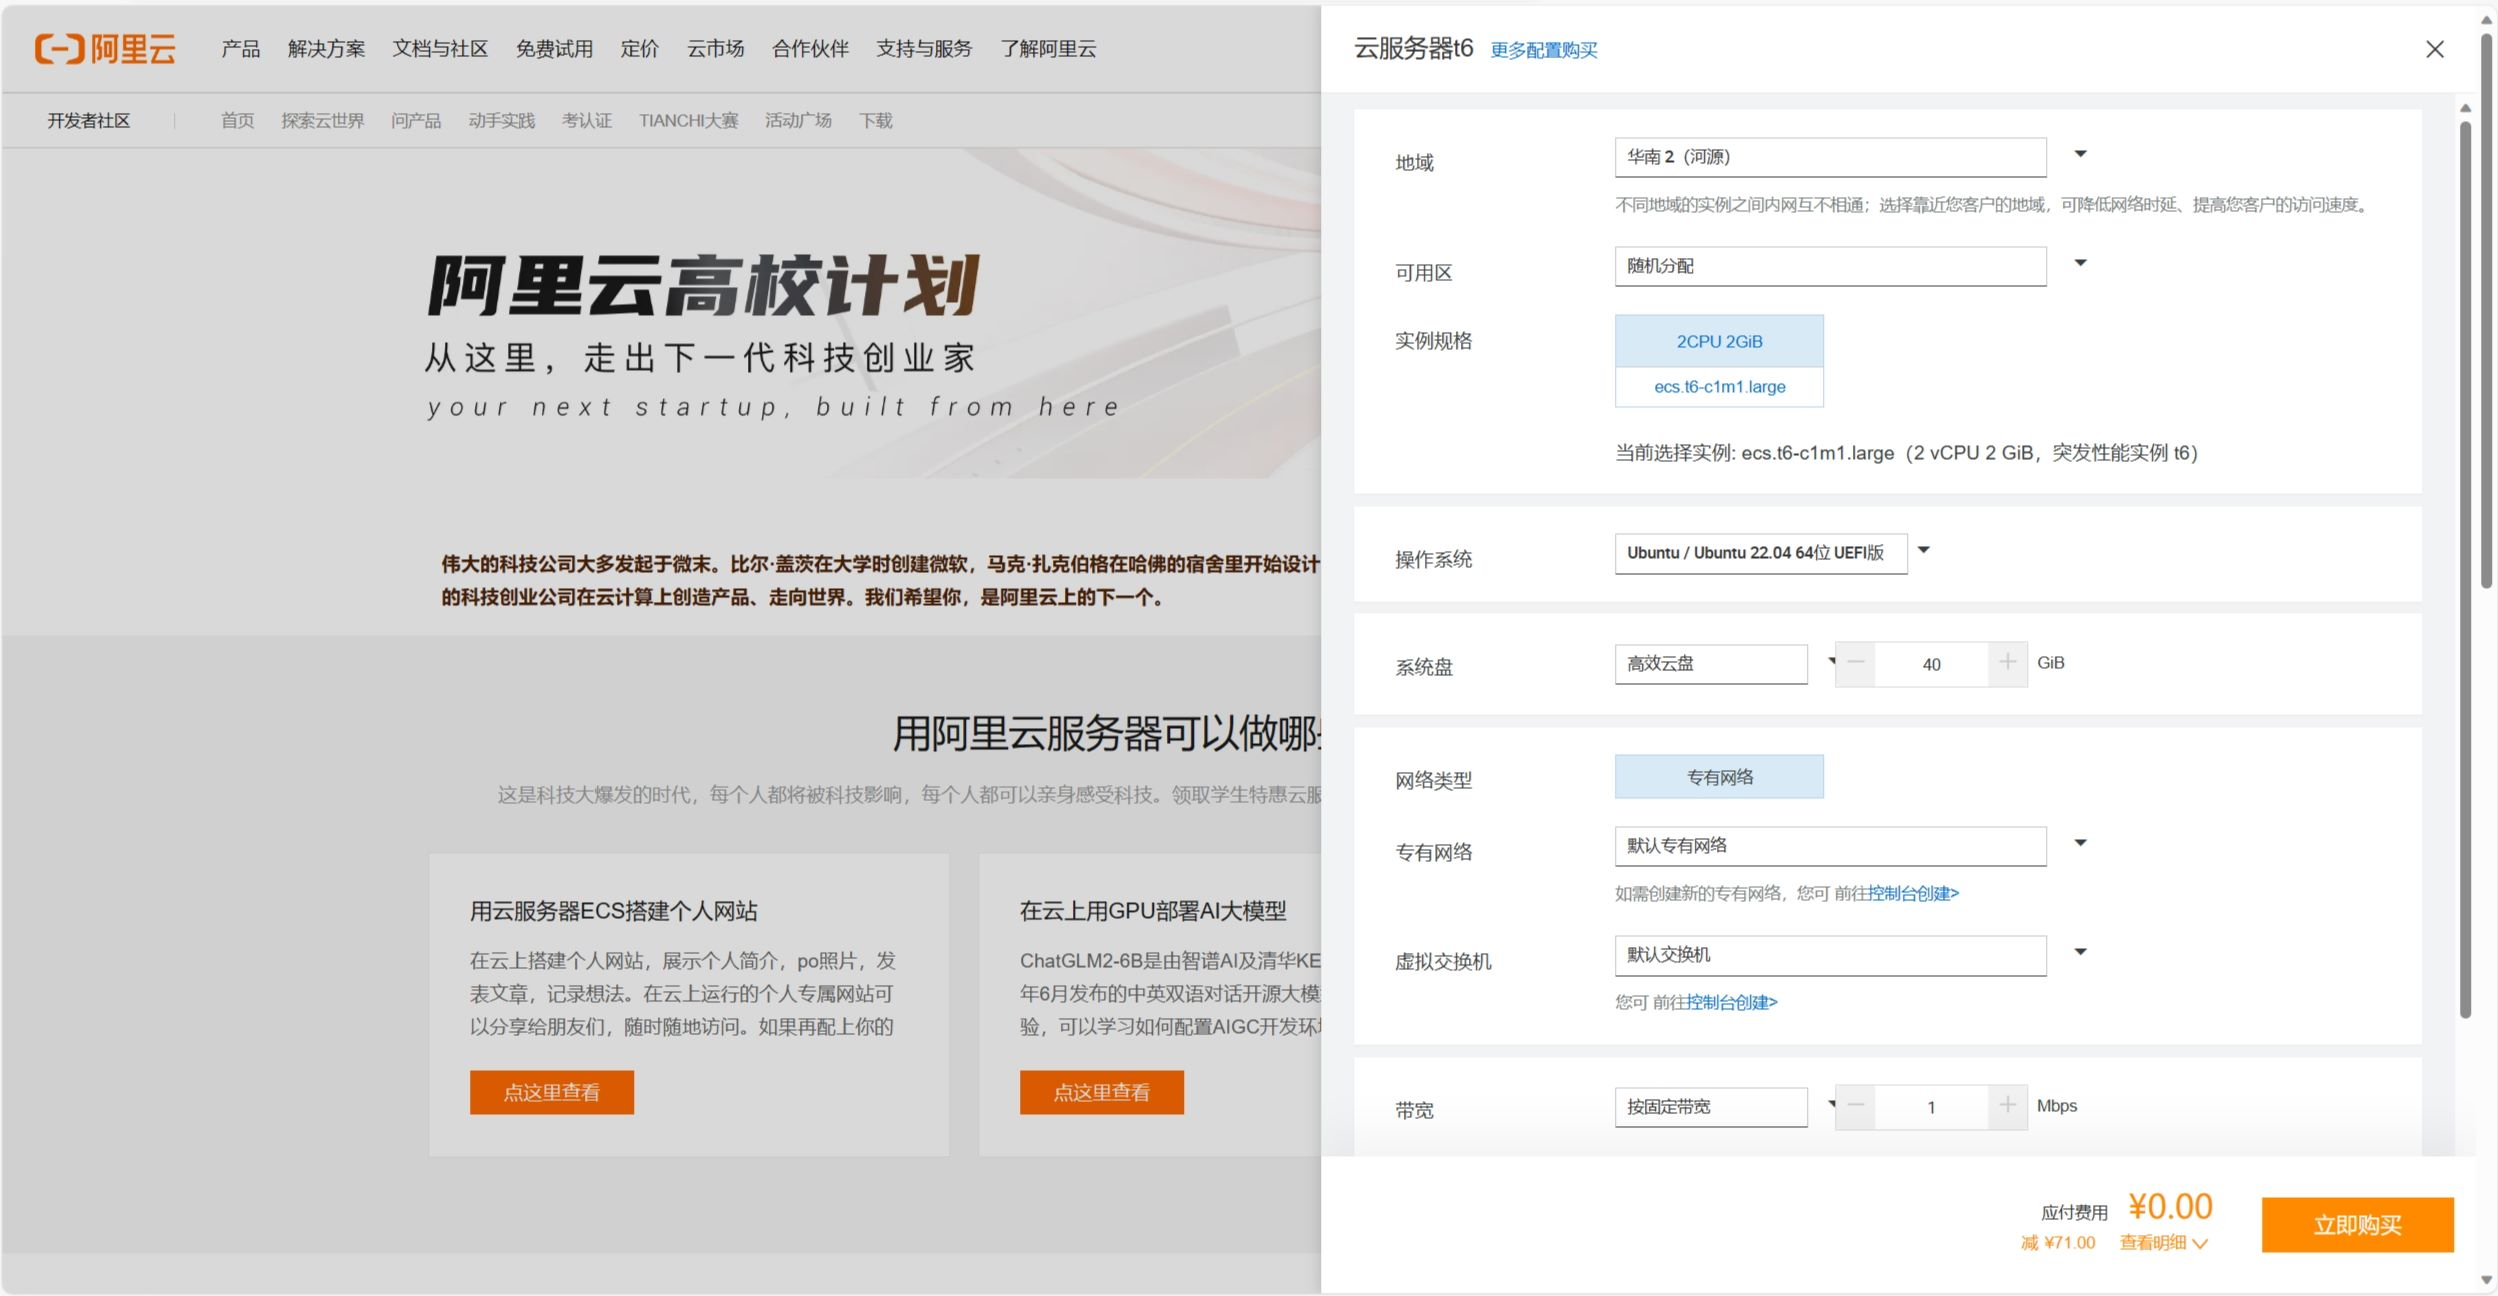
\includegraphics[width=0.7\textwidth]{./pic/1.jpg}
    \caption{注册界面}
\end{figure}
\begin{figure}[H]
    \centering
    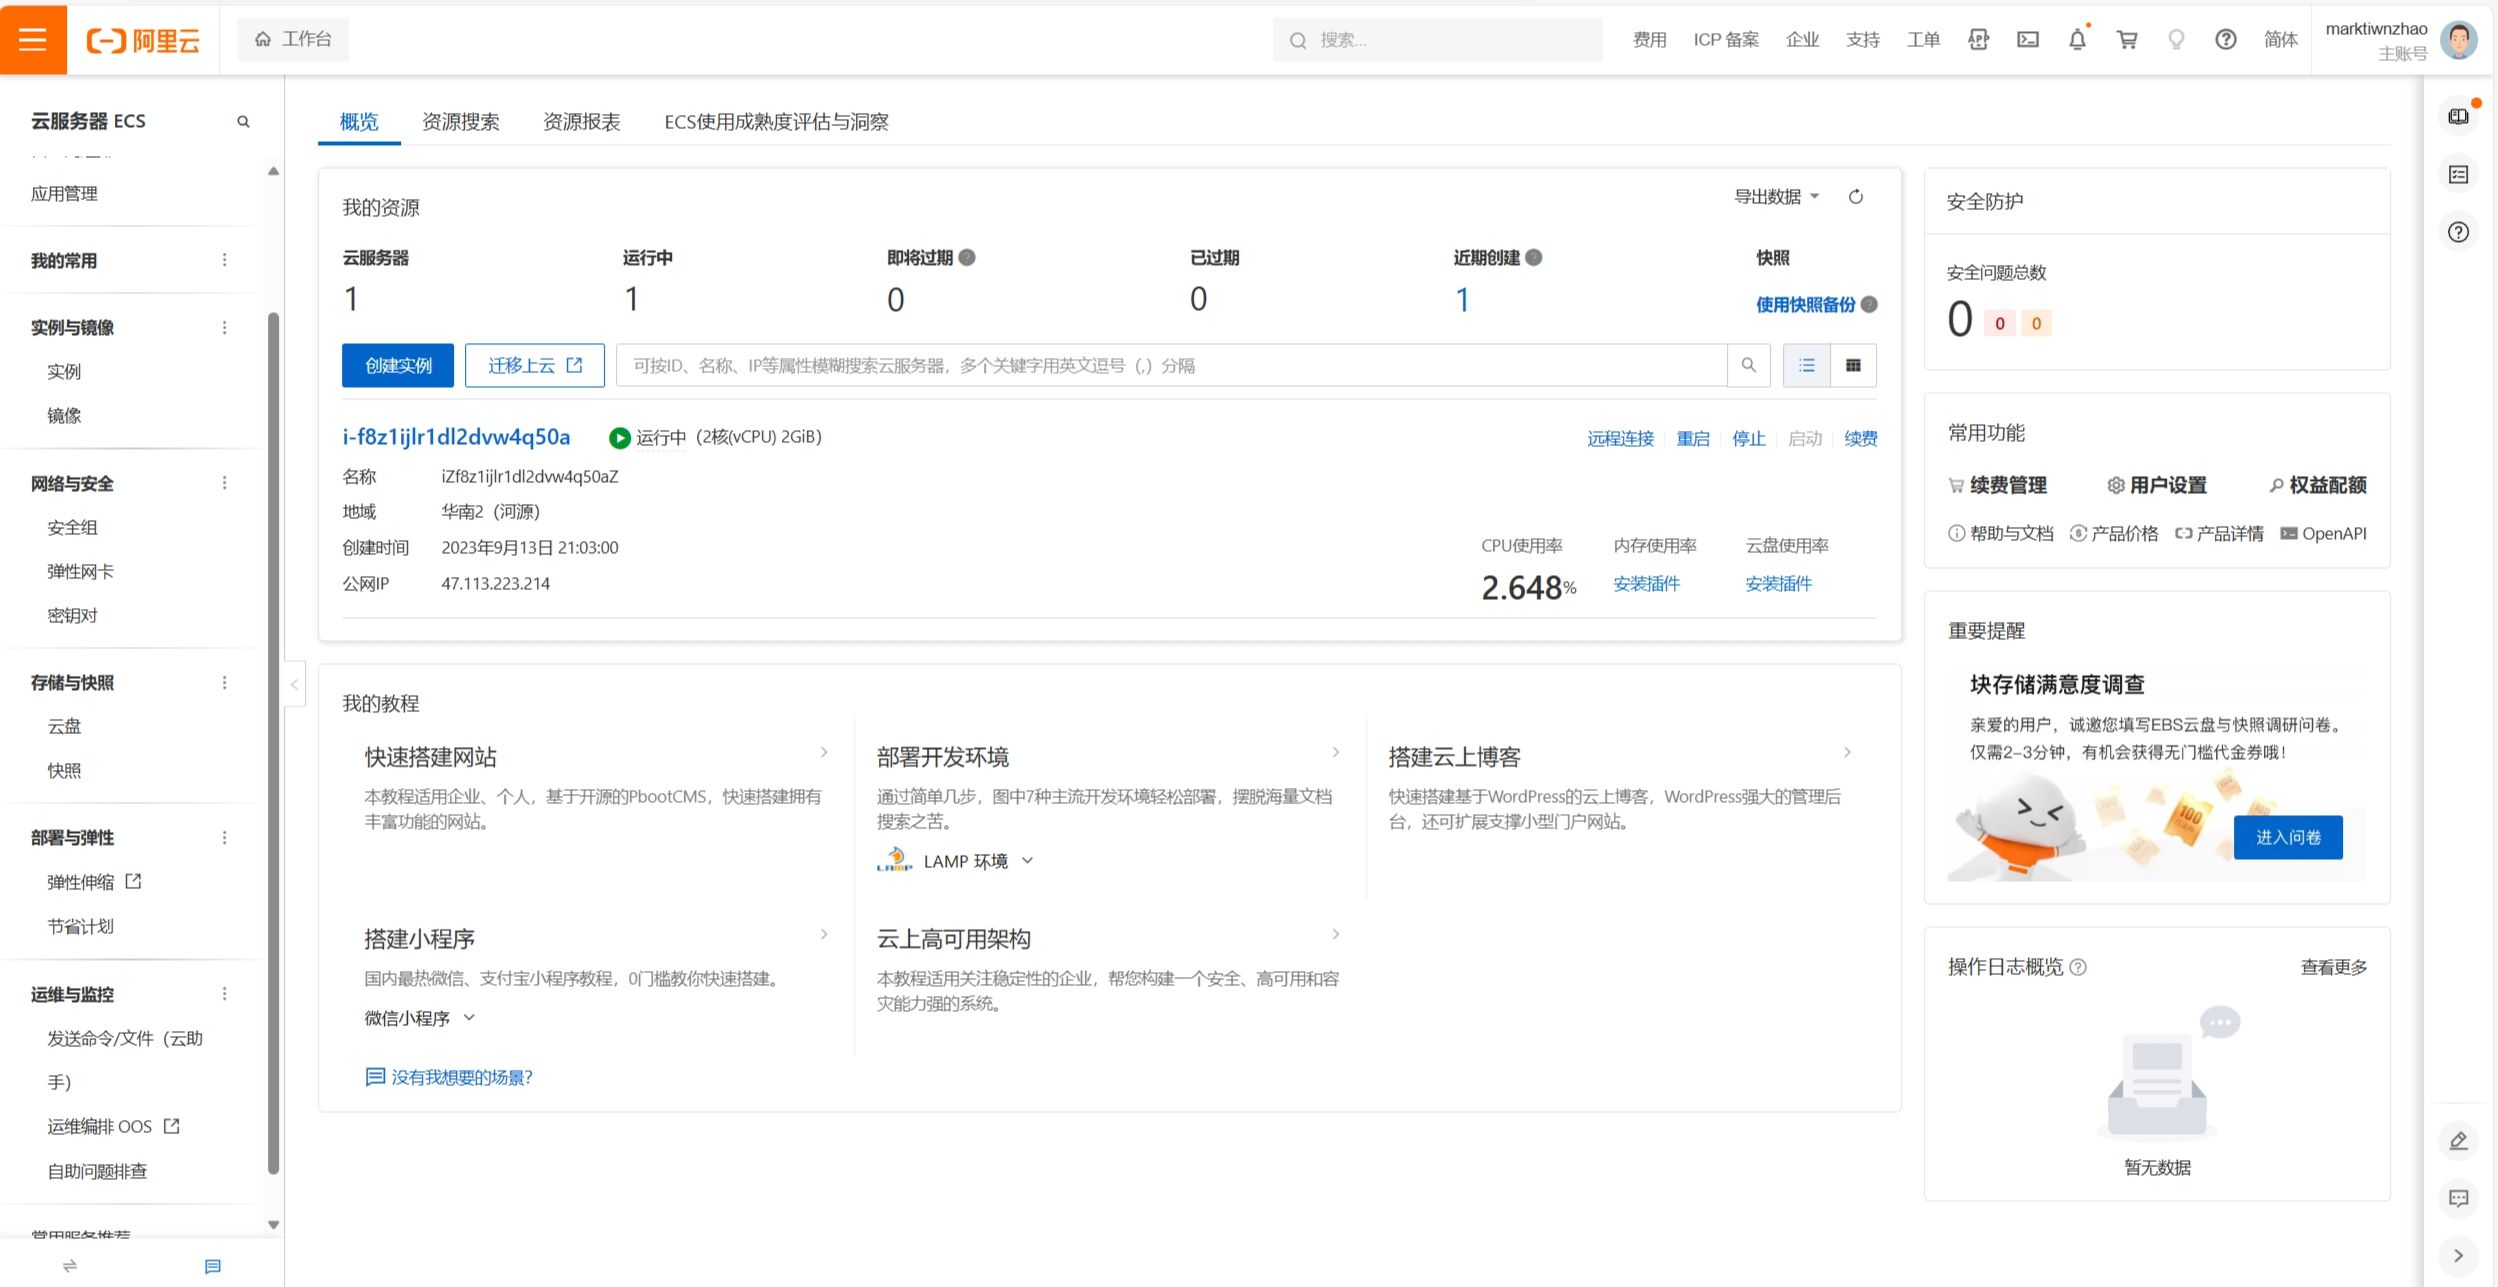
\includegraphics[width=0.7\textwidth]{./pic/2.jpg}
    \caption{控制台界面}
\end{figure}

\subsection*{1.2 安装JDK}
\begin{itemize}
    \item 远程连接已创建的ECS实例,下载JDK1.8安装包并解压。
          \begin{figure}[H]
              \centering
              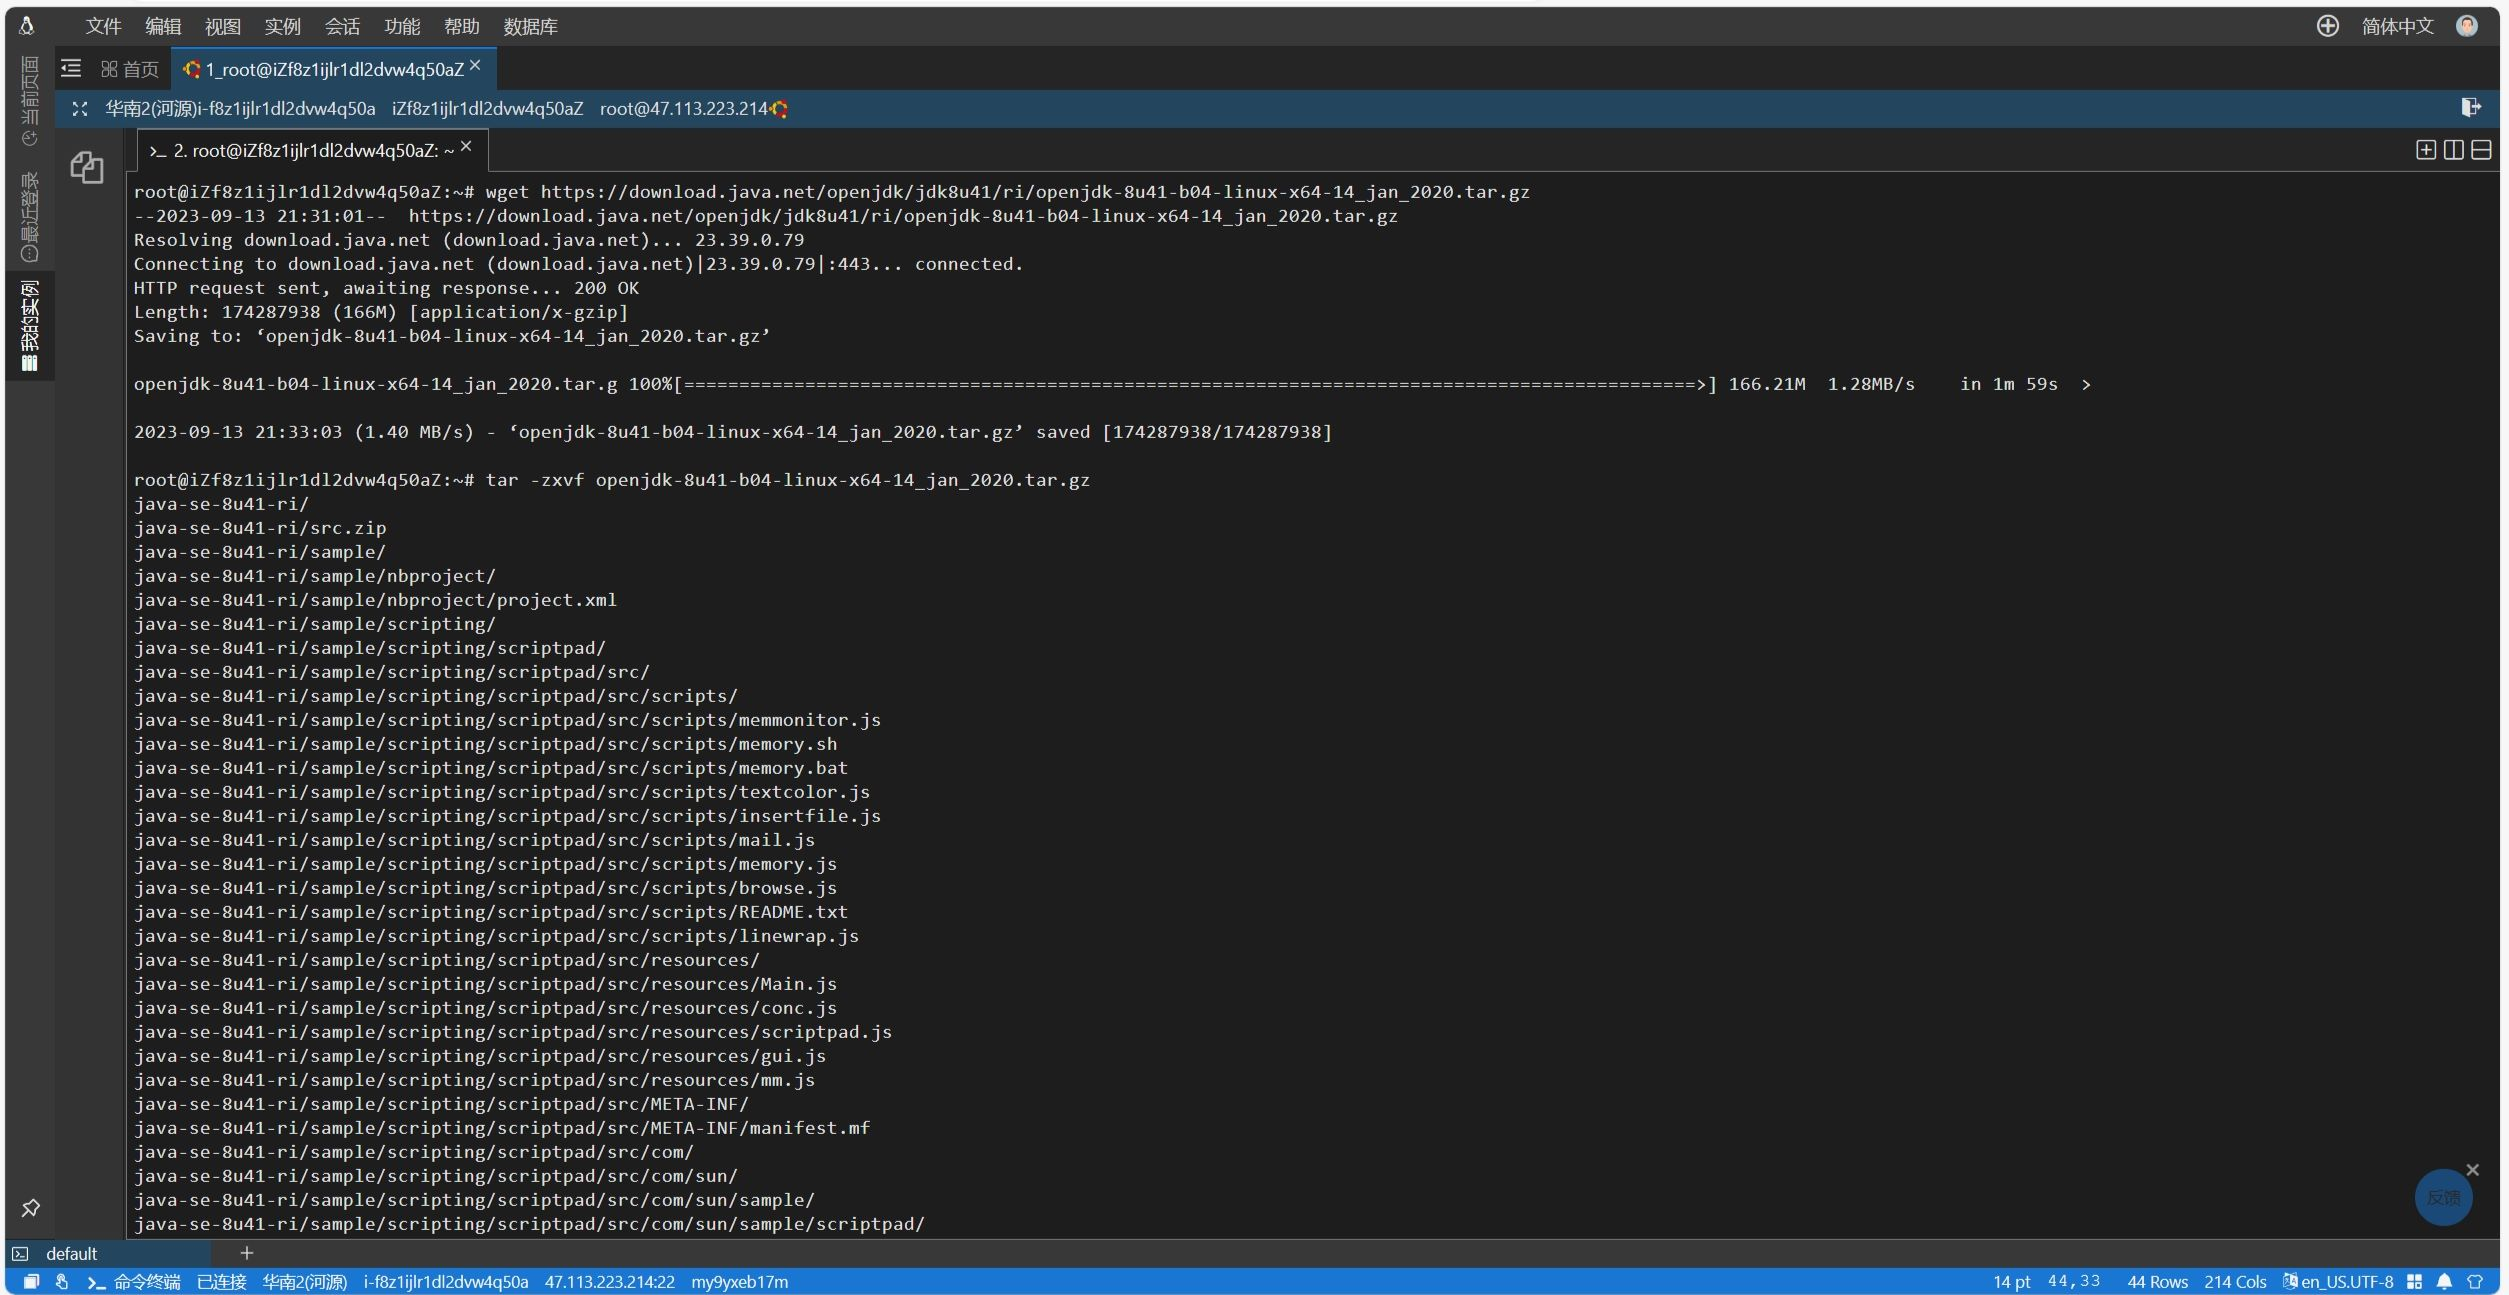
\includegraphics[width=0.7\textwidth]{./pic/3.jpg}
              \caption{下载并解压JDK}
          \end{figure}
    \item 解压完成后,移动JDK安装包至/usr/java8。之后配置Java环境变量。完成后查看Java版本。
          \begin{figure}[H]
              \centering
              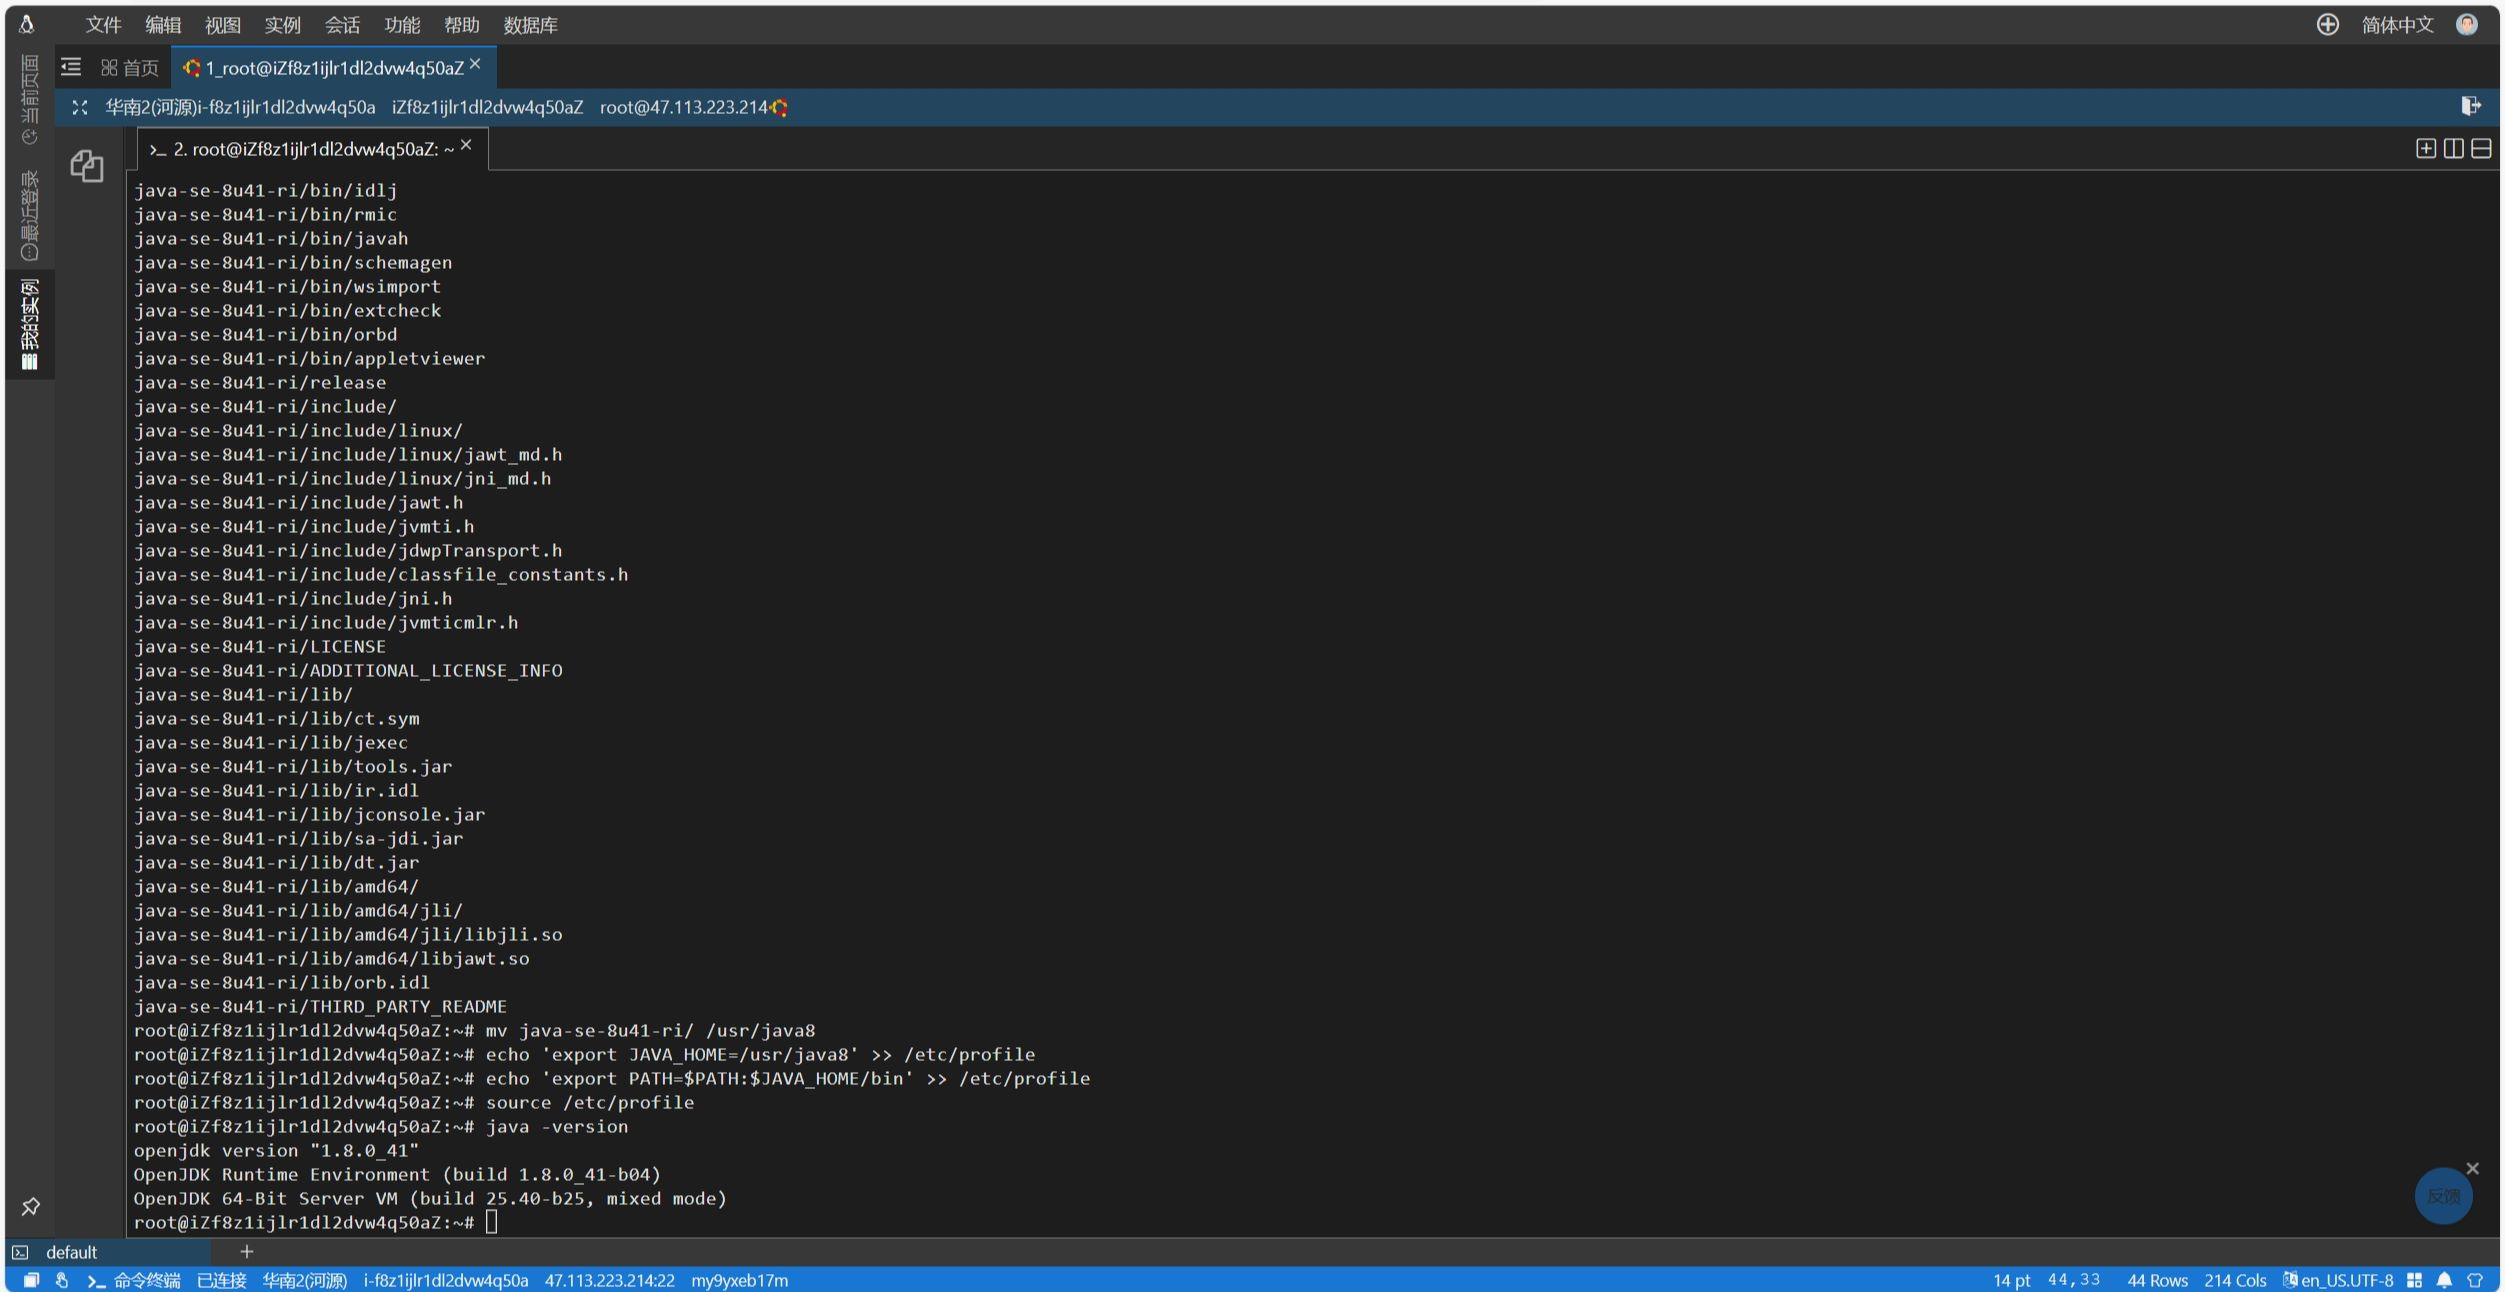
\includegraphics[width=0.7\textwidth]{./pic/4.jpg}
              \caption{配置环境变量}
          \end{figure}
\end{itemize}

\subsection*{1.3 搭建Hadoop环境}
\begin{itemize}
    \item 下载Hadoop安装包。
          \begin{figure}[H]
              \centering
              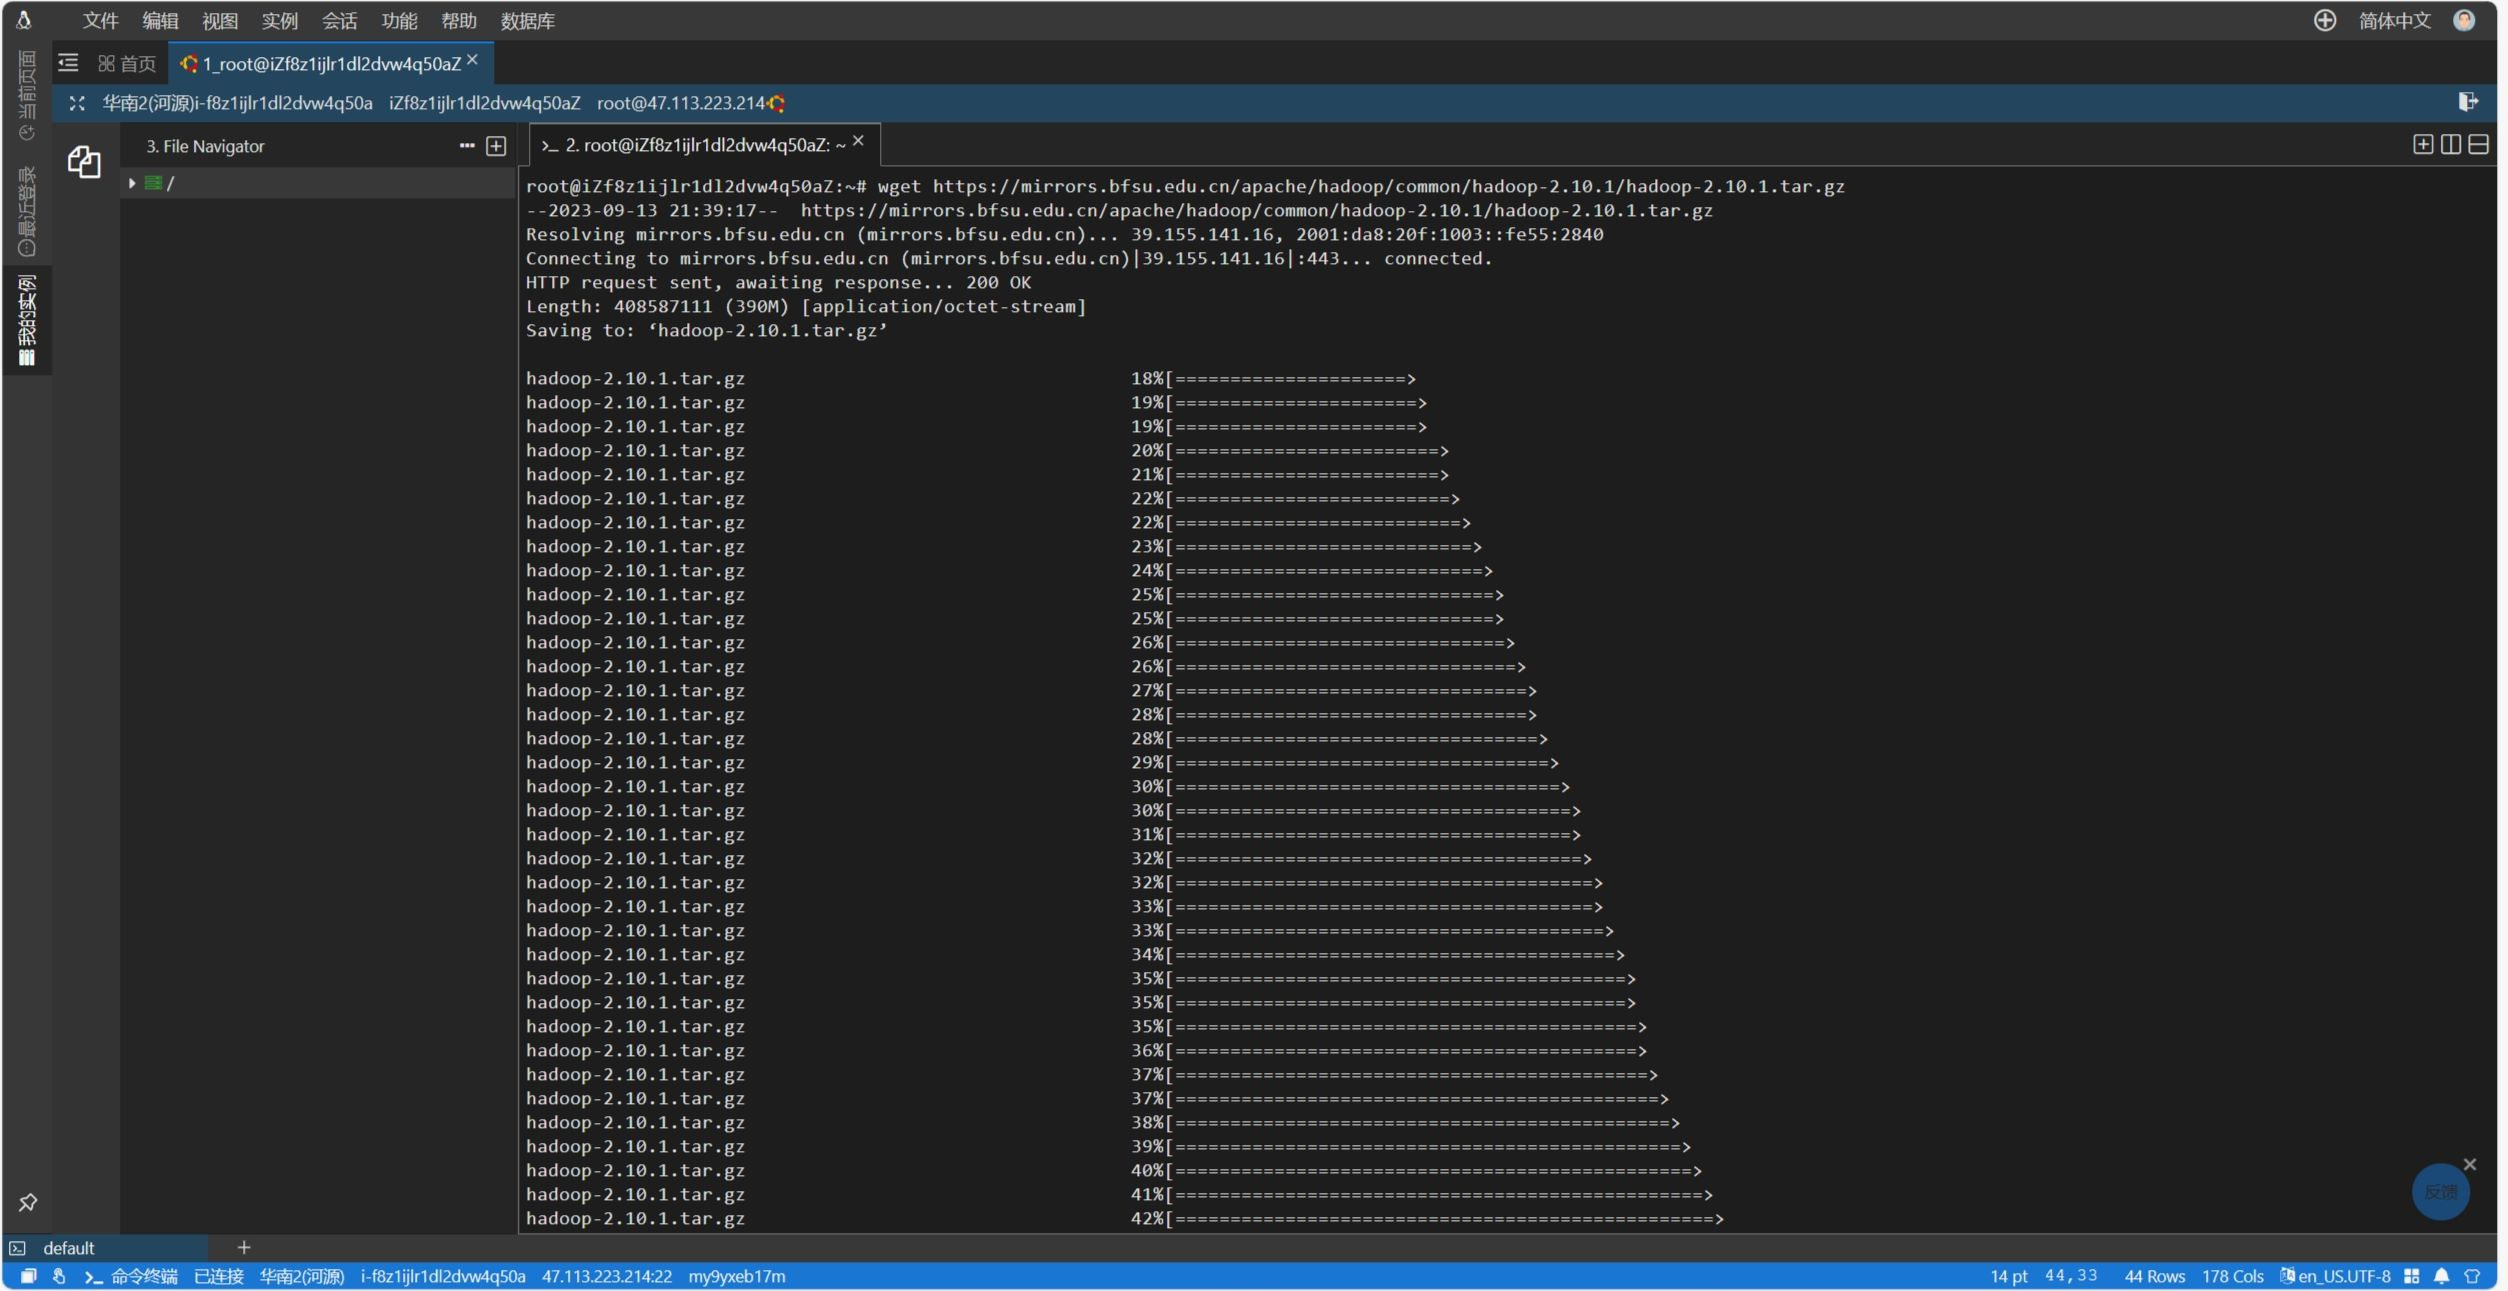
\includegraphics[width=0.7\textwidth]{./pic/5.jpg}
              \caption{下载Hadoop}
          \end{figure}
    \item 解压Hadoop安装包至/opt/hadoop。之后配置Hadoop环境变量并修改配置文件yarn-env.sh和hadoop-env.sh。完成后查看hadoop版本。
          \begin{figure}[H]
              \centering
              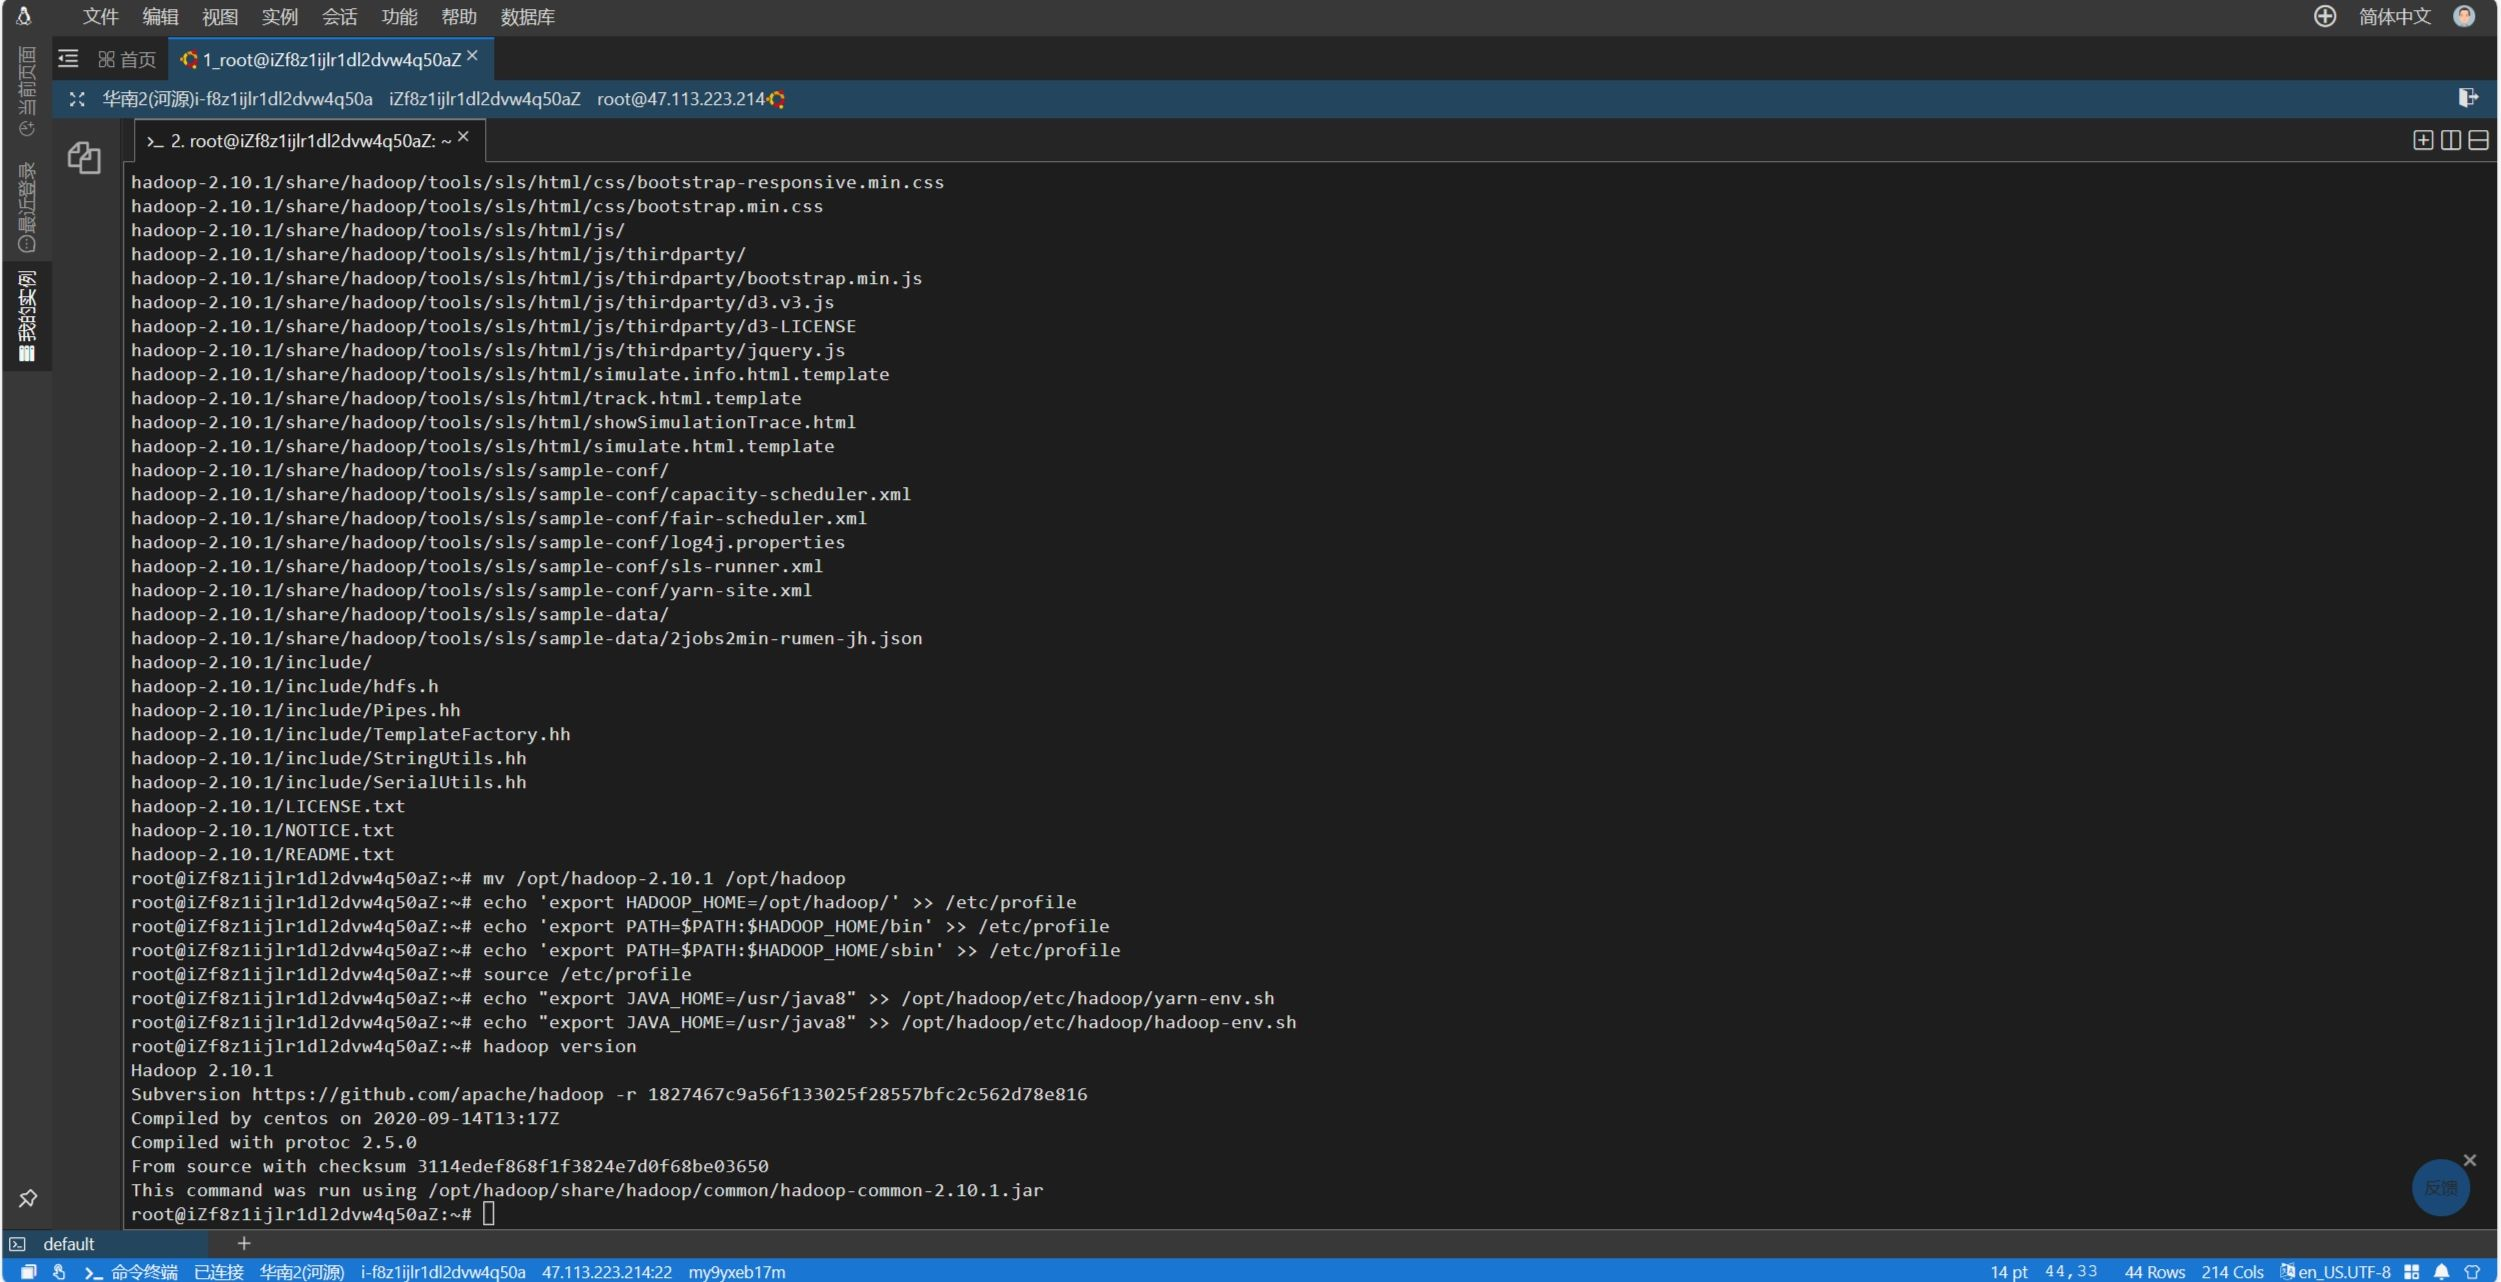
\includegraphics[width=0.7\textwidth]{./pic/6.jpg}
              \caption{配置环境变量并修改配置文件}
          \end{figure}
    \item 修改Hadoop配置文件core-site.xml和hdfs-site.xml。
          \begin{figure}[H]
              \centering
              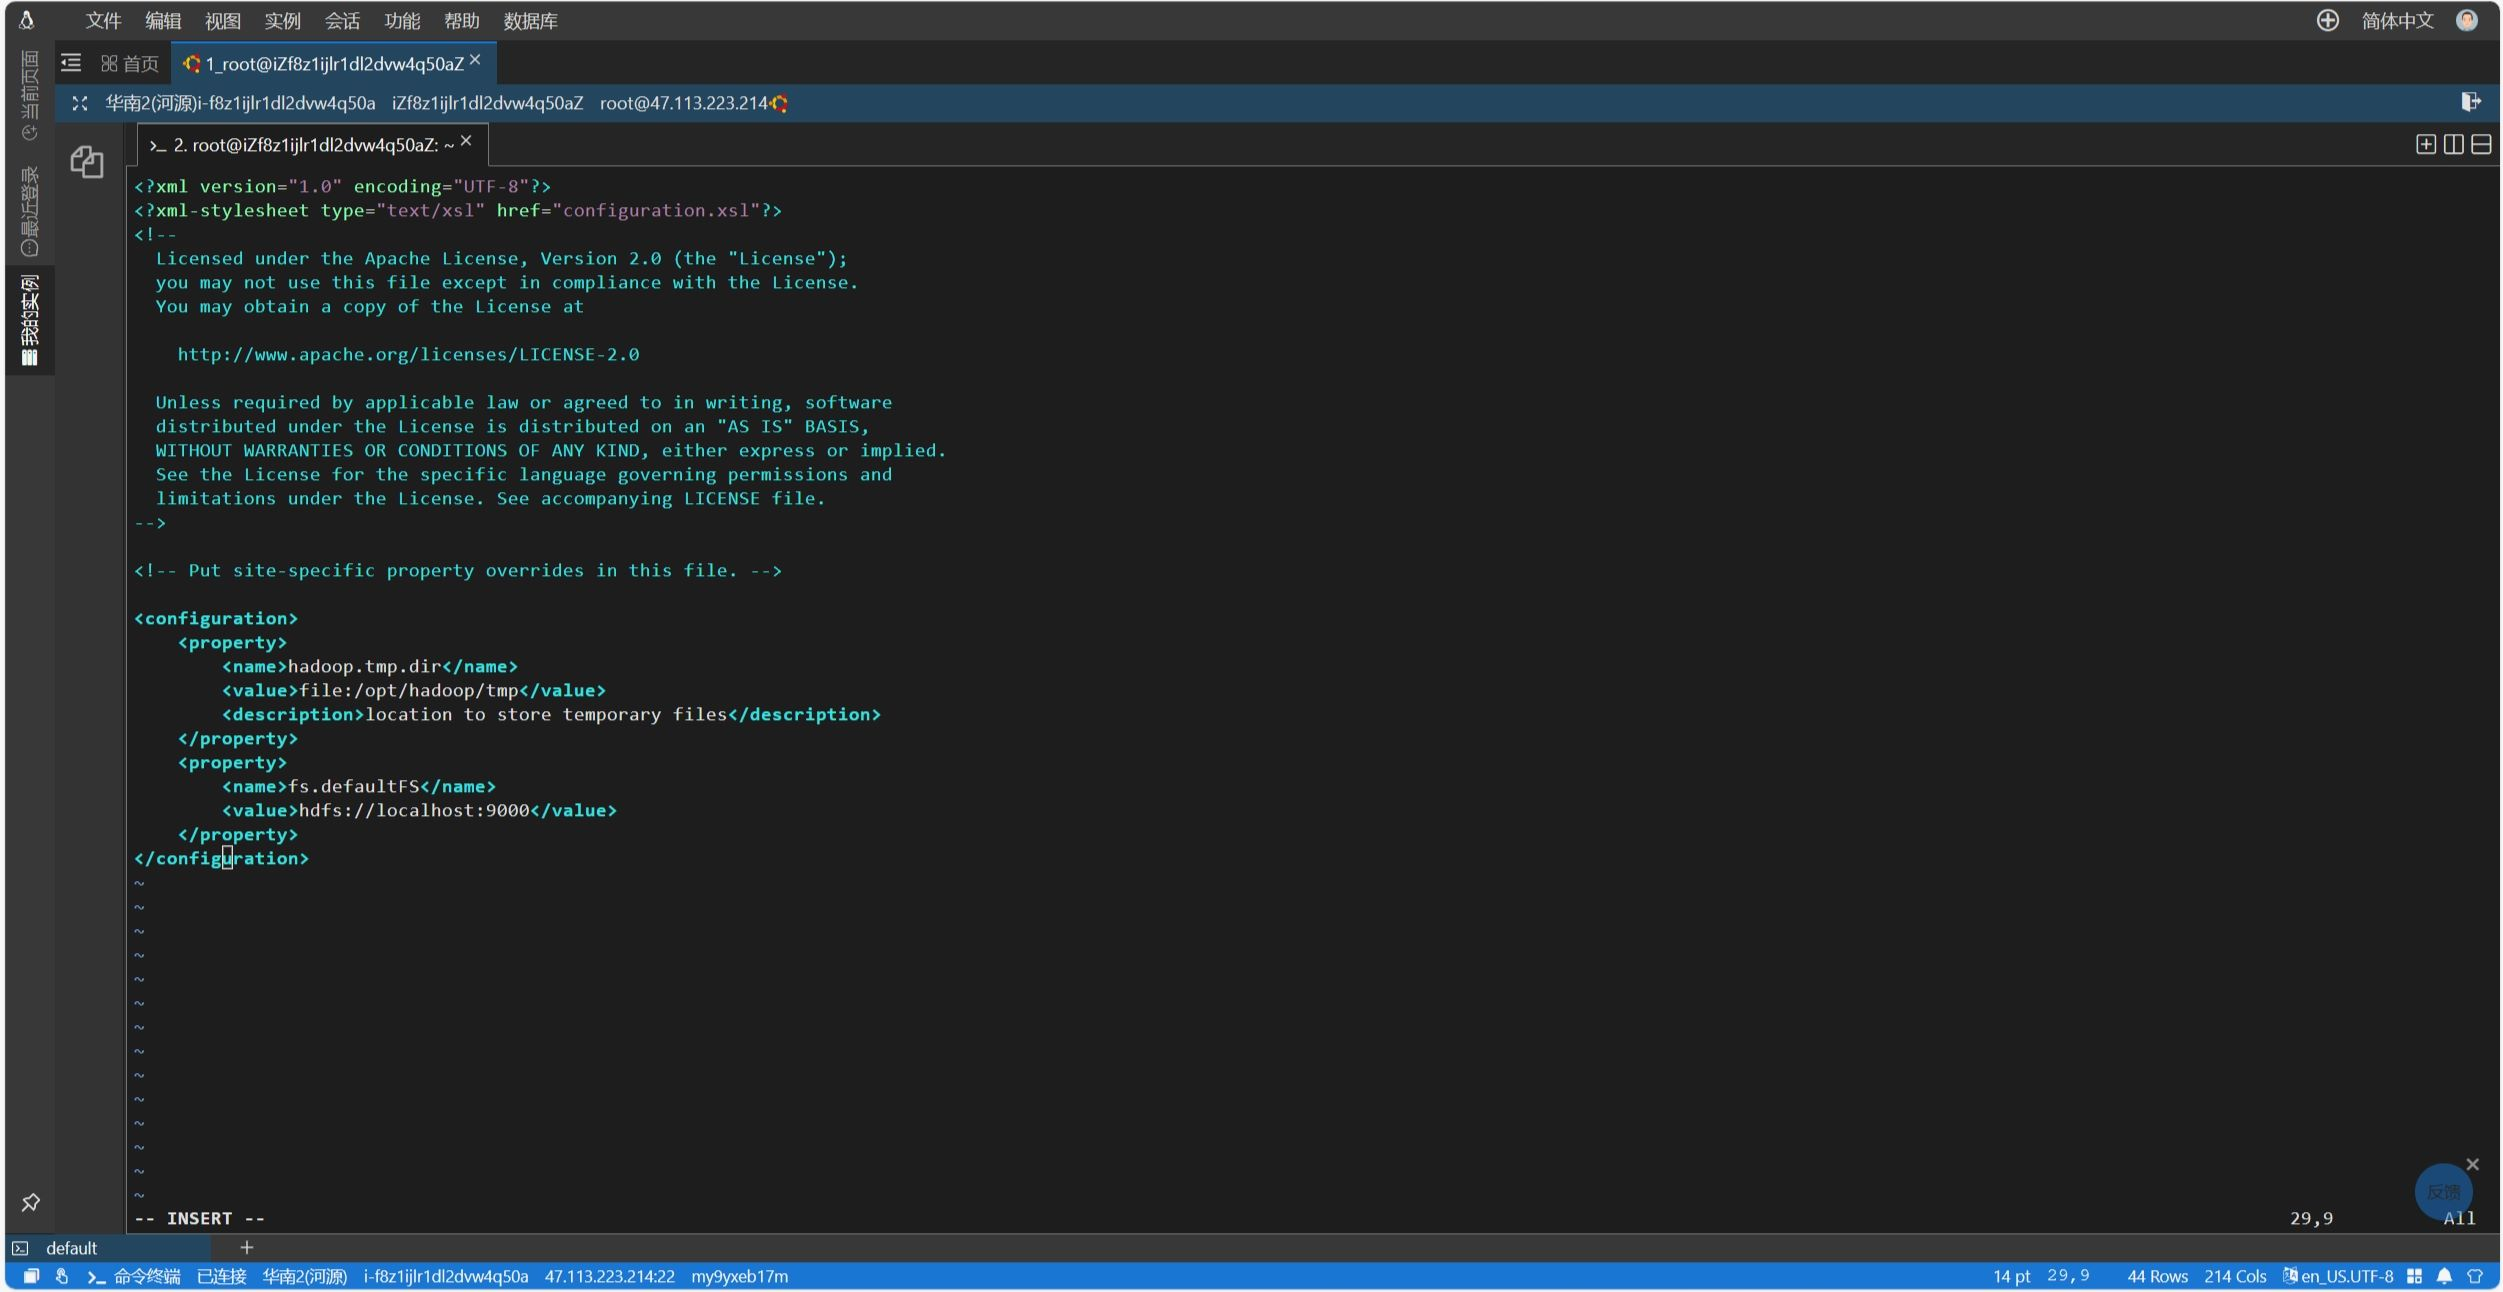
\includegraphics[width=0.7\textwidth]{./pic/7.jpg}
              \caption{core-site.xml}
          \end{figure}
          \begin{figure}[H]
              \centering
              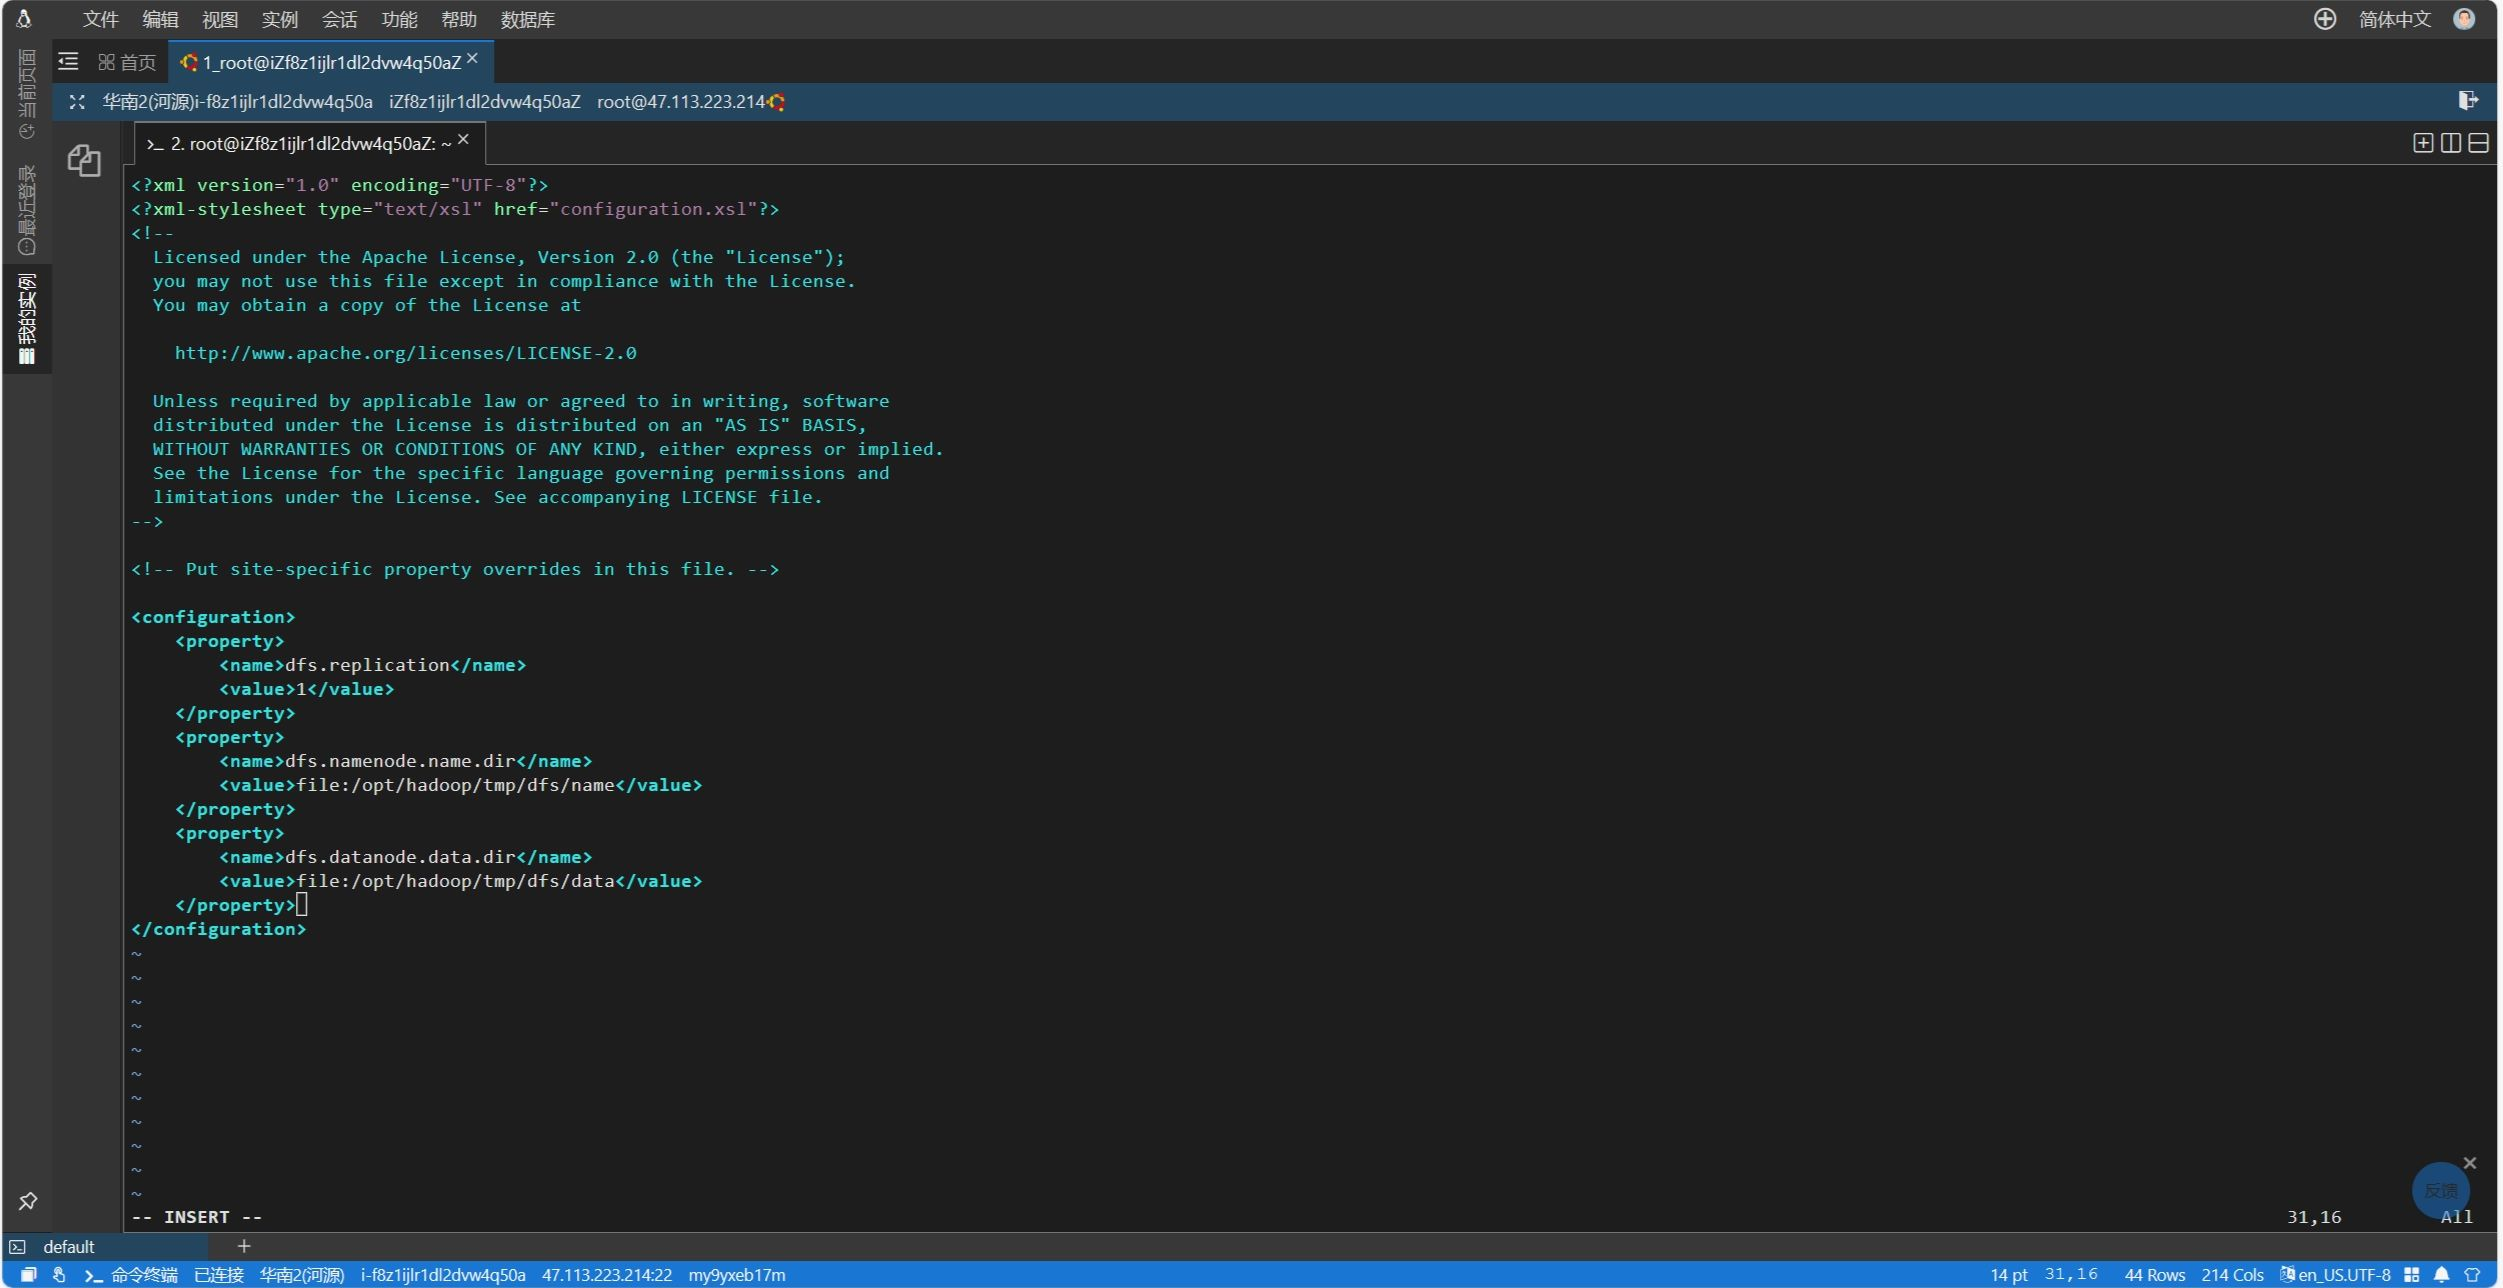
\includegraphics[width=0.7\textwidth]{./pic/8.jpg}
              \caption{hdfs-site.xml}
          \end{figure}
    \item 配置SSH免密登录:创建公钥和私钥,并将公钥添加到authorized\_keys文件中。
          \begin{figure}[H]
              \centering
              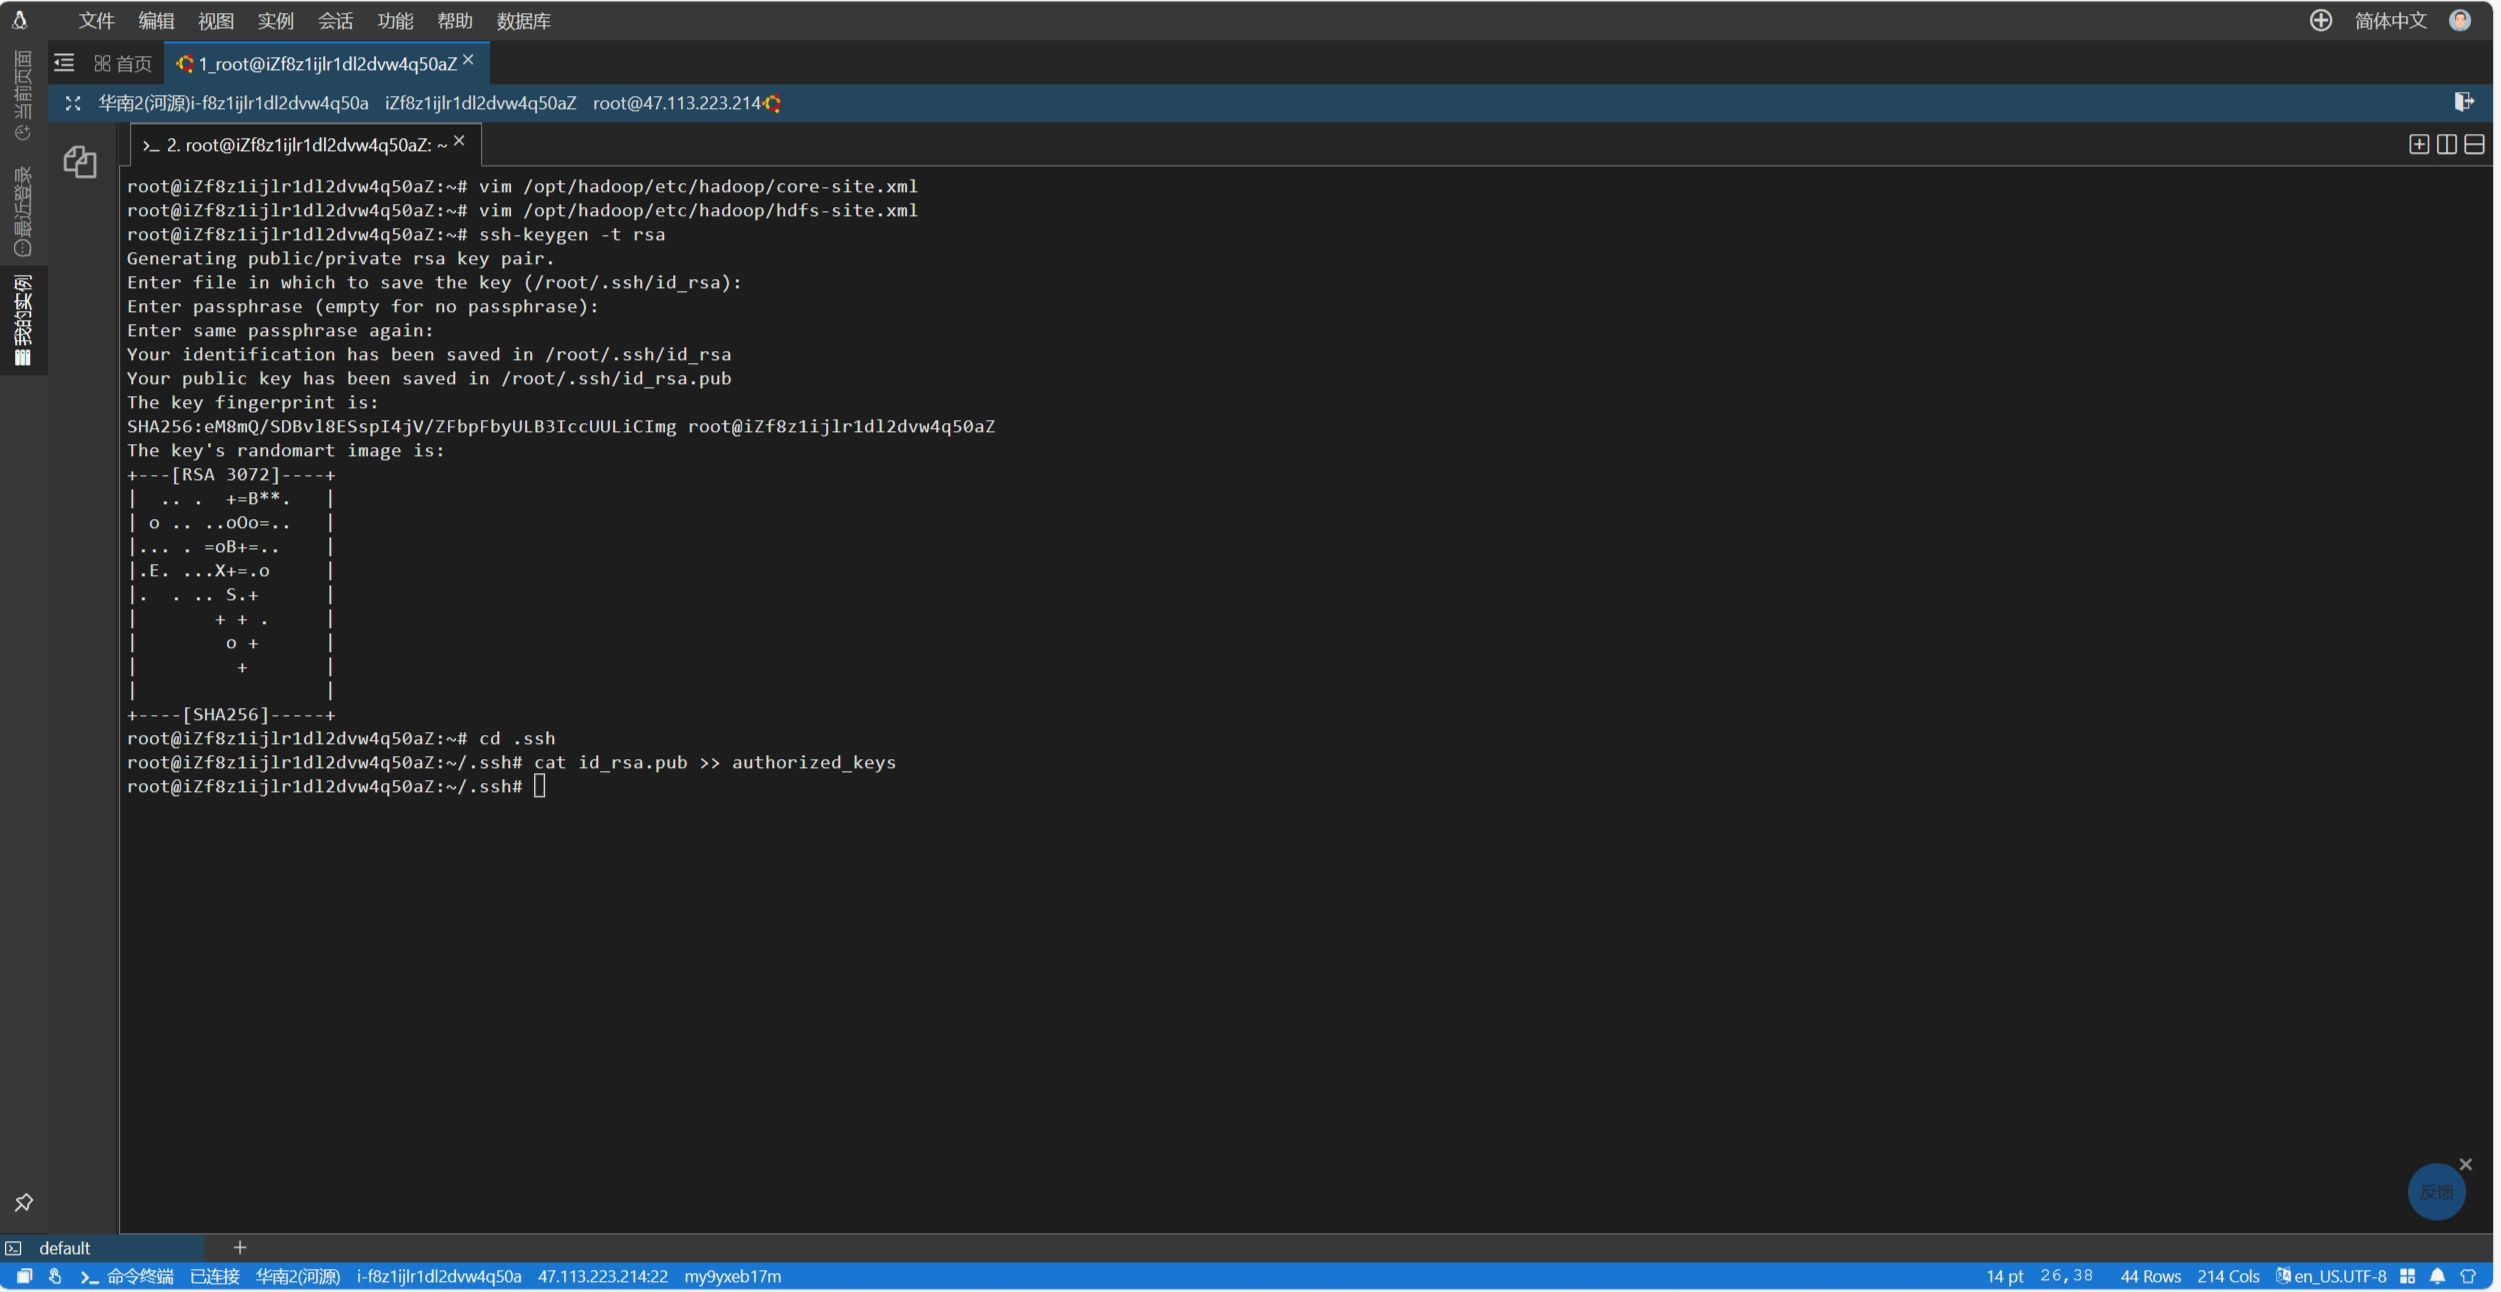
\includegraphics[width=0.7\textwidth]{./pic/9.jpg}
              \caption{hdfs-site.xml}
          \end{figure}
    \item 通过\lstinline[language=bash]|start-all.sh|启动Hadoop,通过\lstinline[language=bash]|jps|查看成功启动的进程。
          \begin{figure}[H]
              \centering
              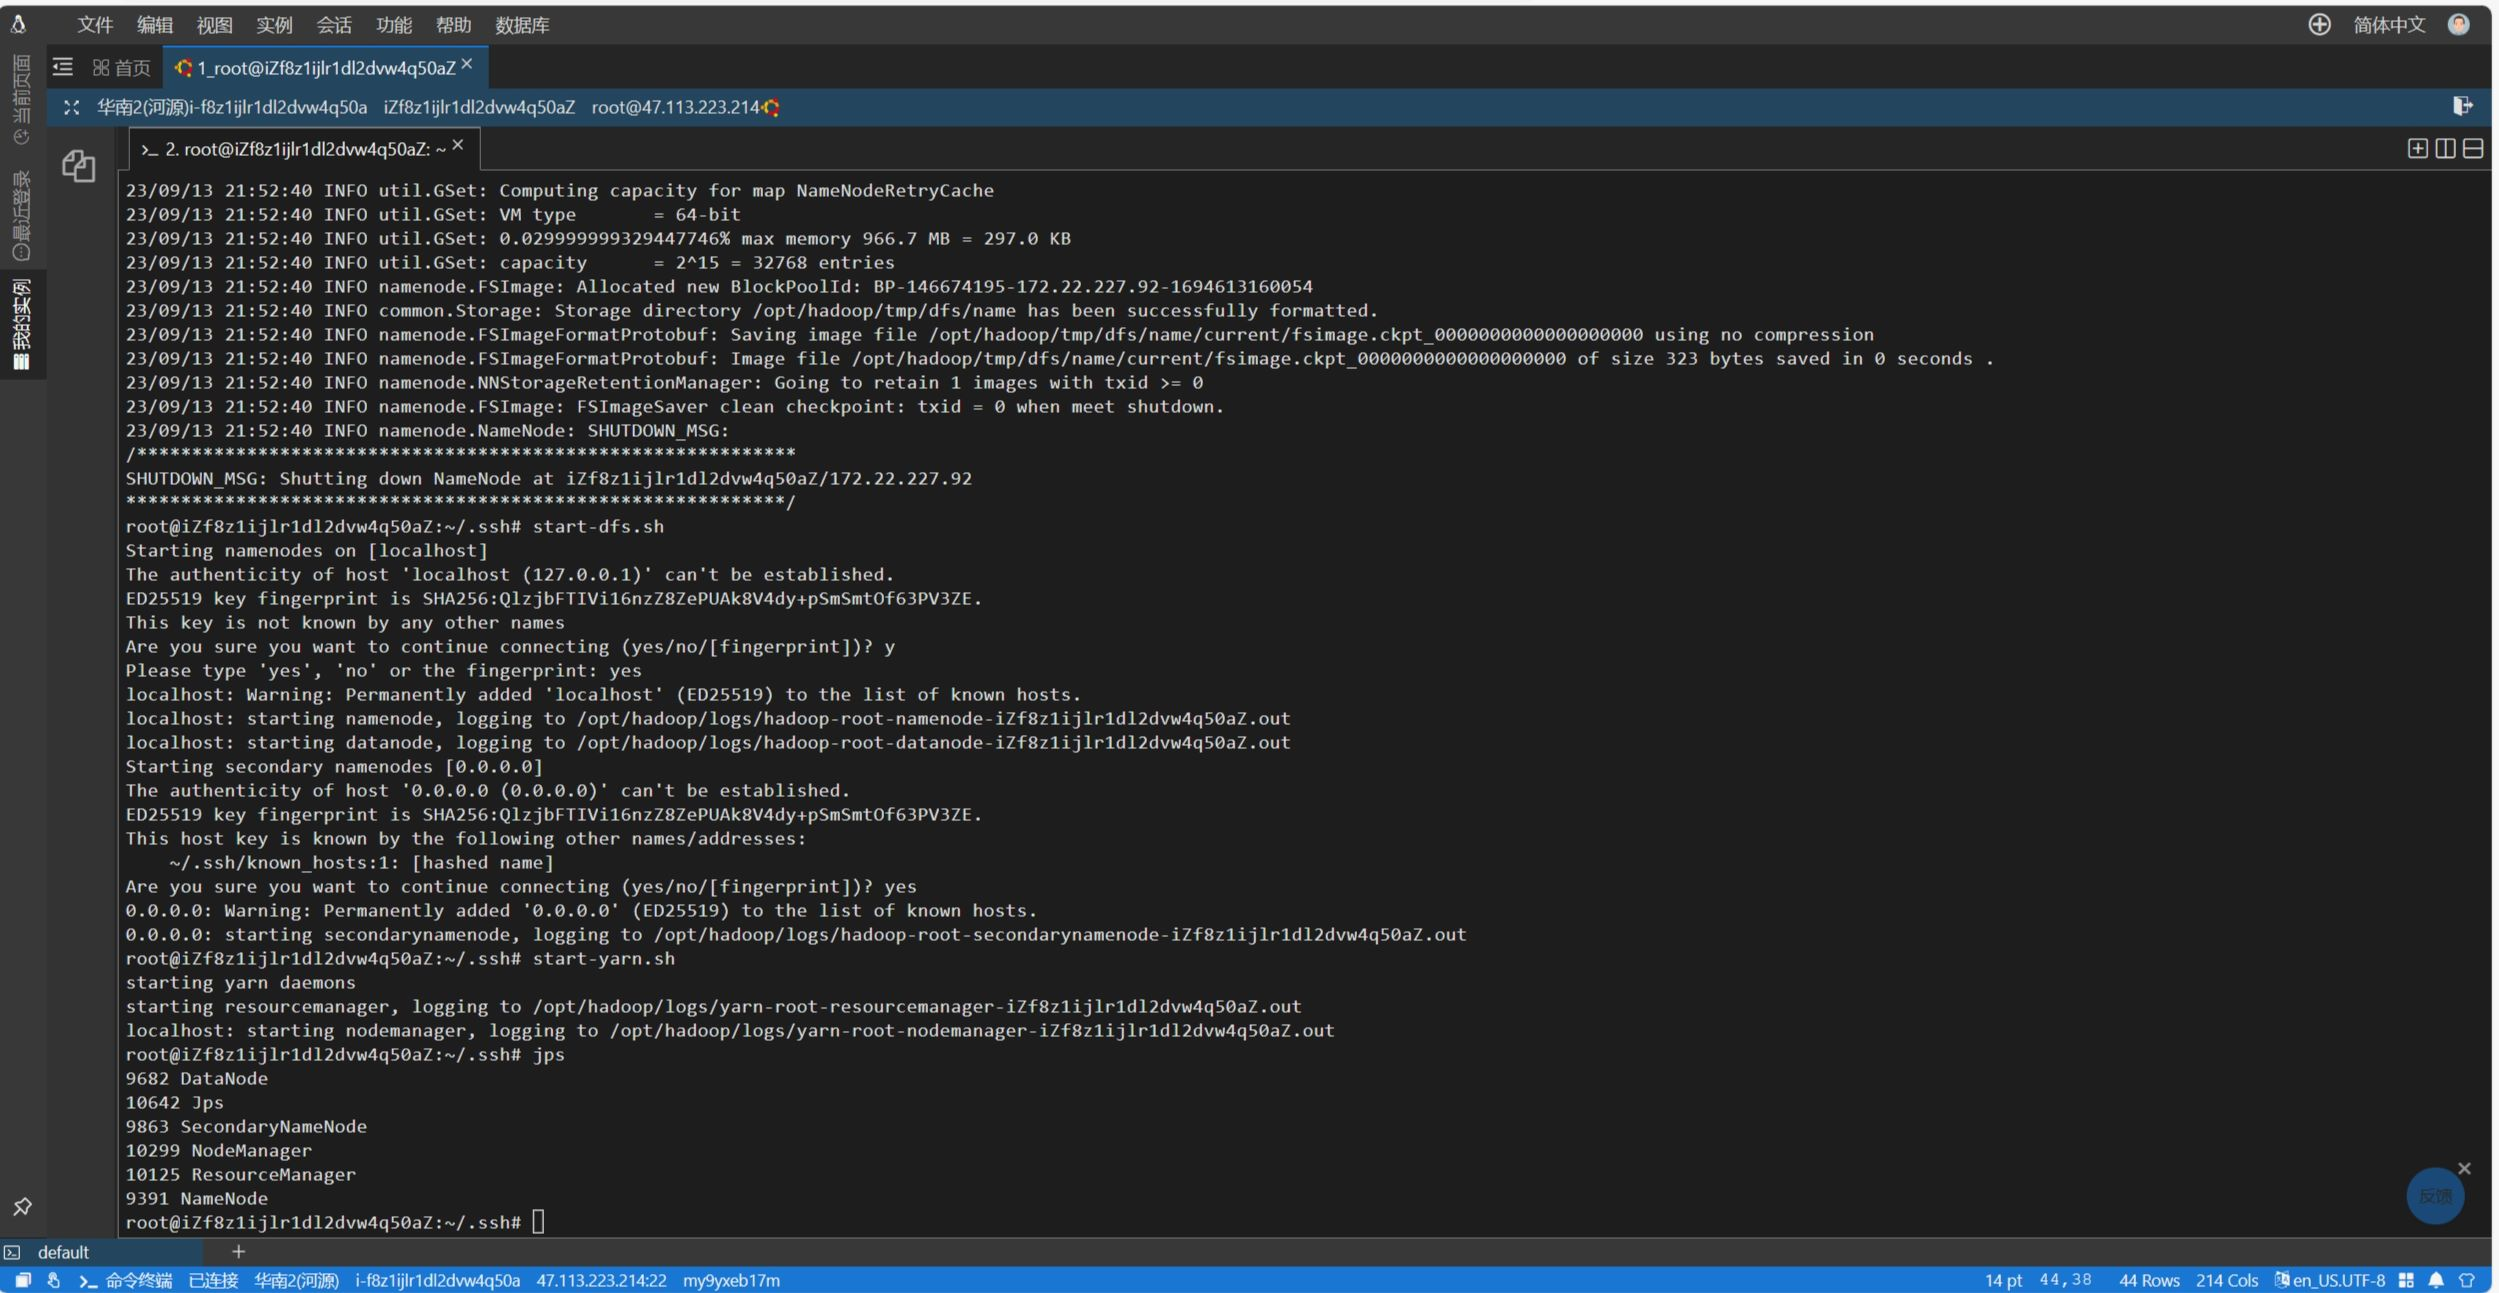
\includegraphics[width=0.7\textwidth]{./pic/10.jpg}
              \caption{启动Hadoop}
          \end{figure}
    \item 通过浏览器查看Hadoop的Web界面。
          \begin{figure}[H]
              \centering
              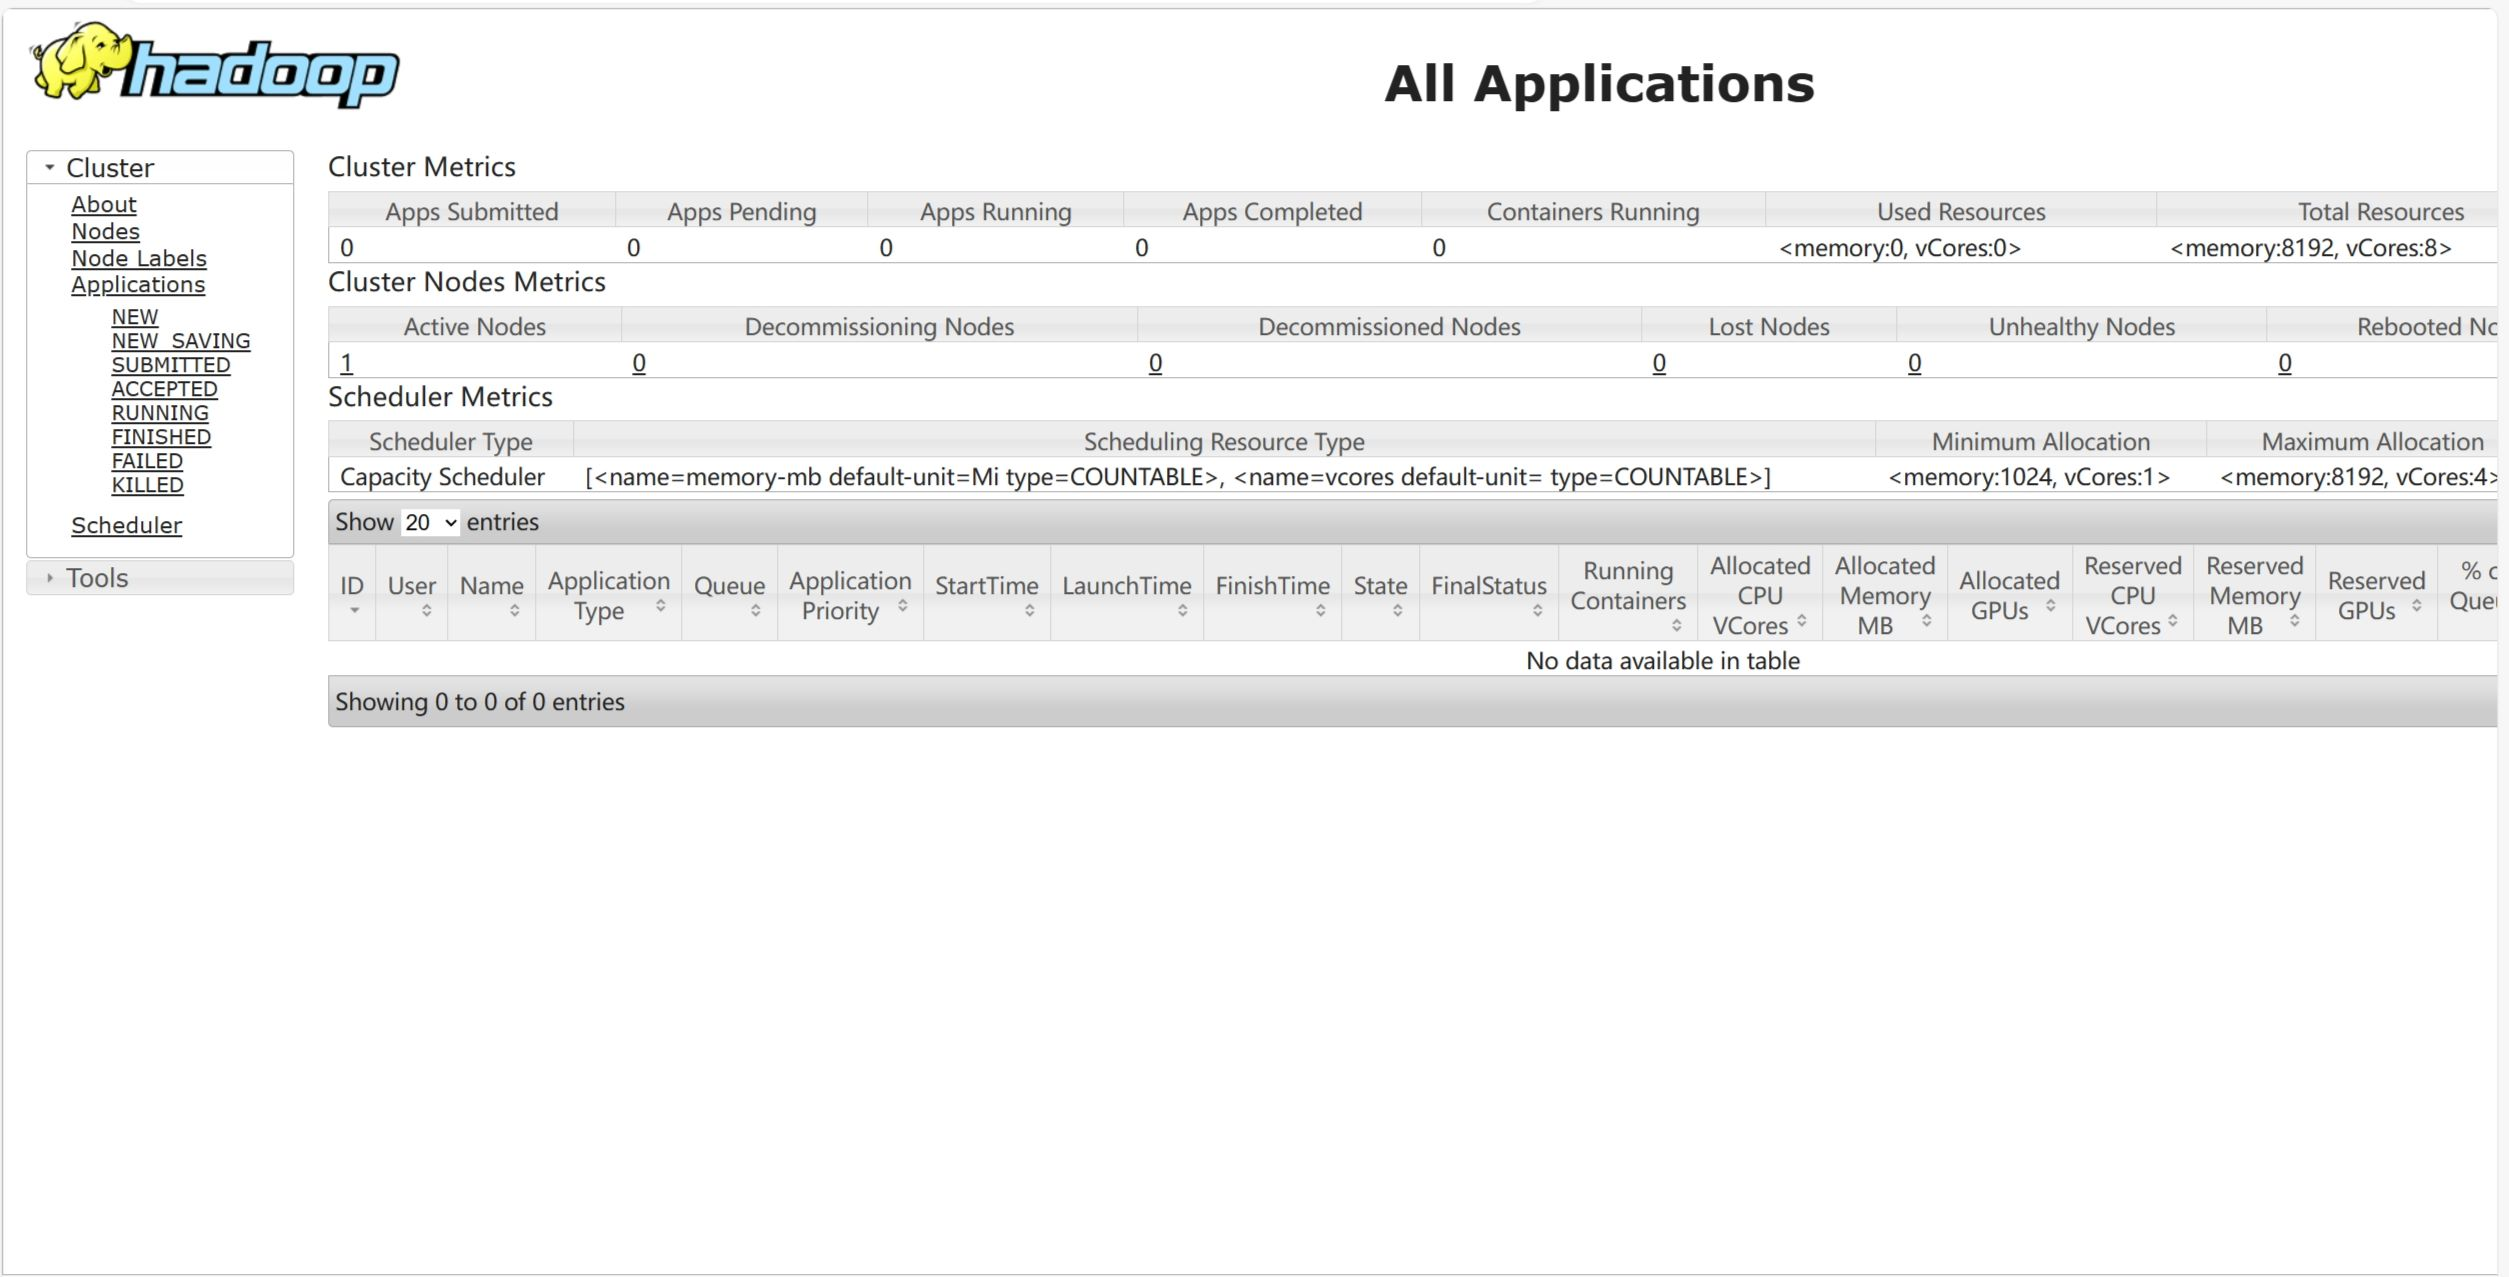
\includegraphics[width=0.7\textwidth]{./pic/11.jpg}
              \caption{8088端口}
          \end{figure}
          \begin{figure}[H]
              \centering
              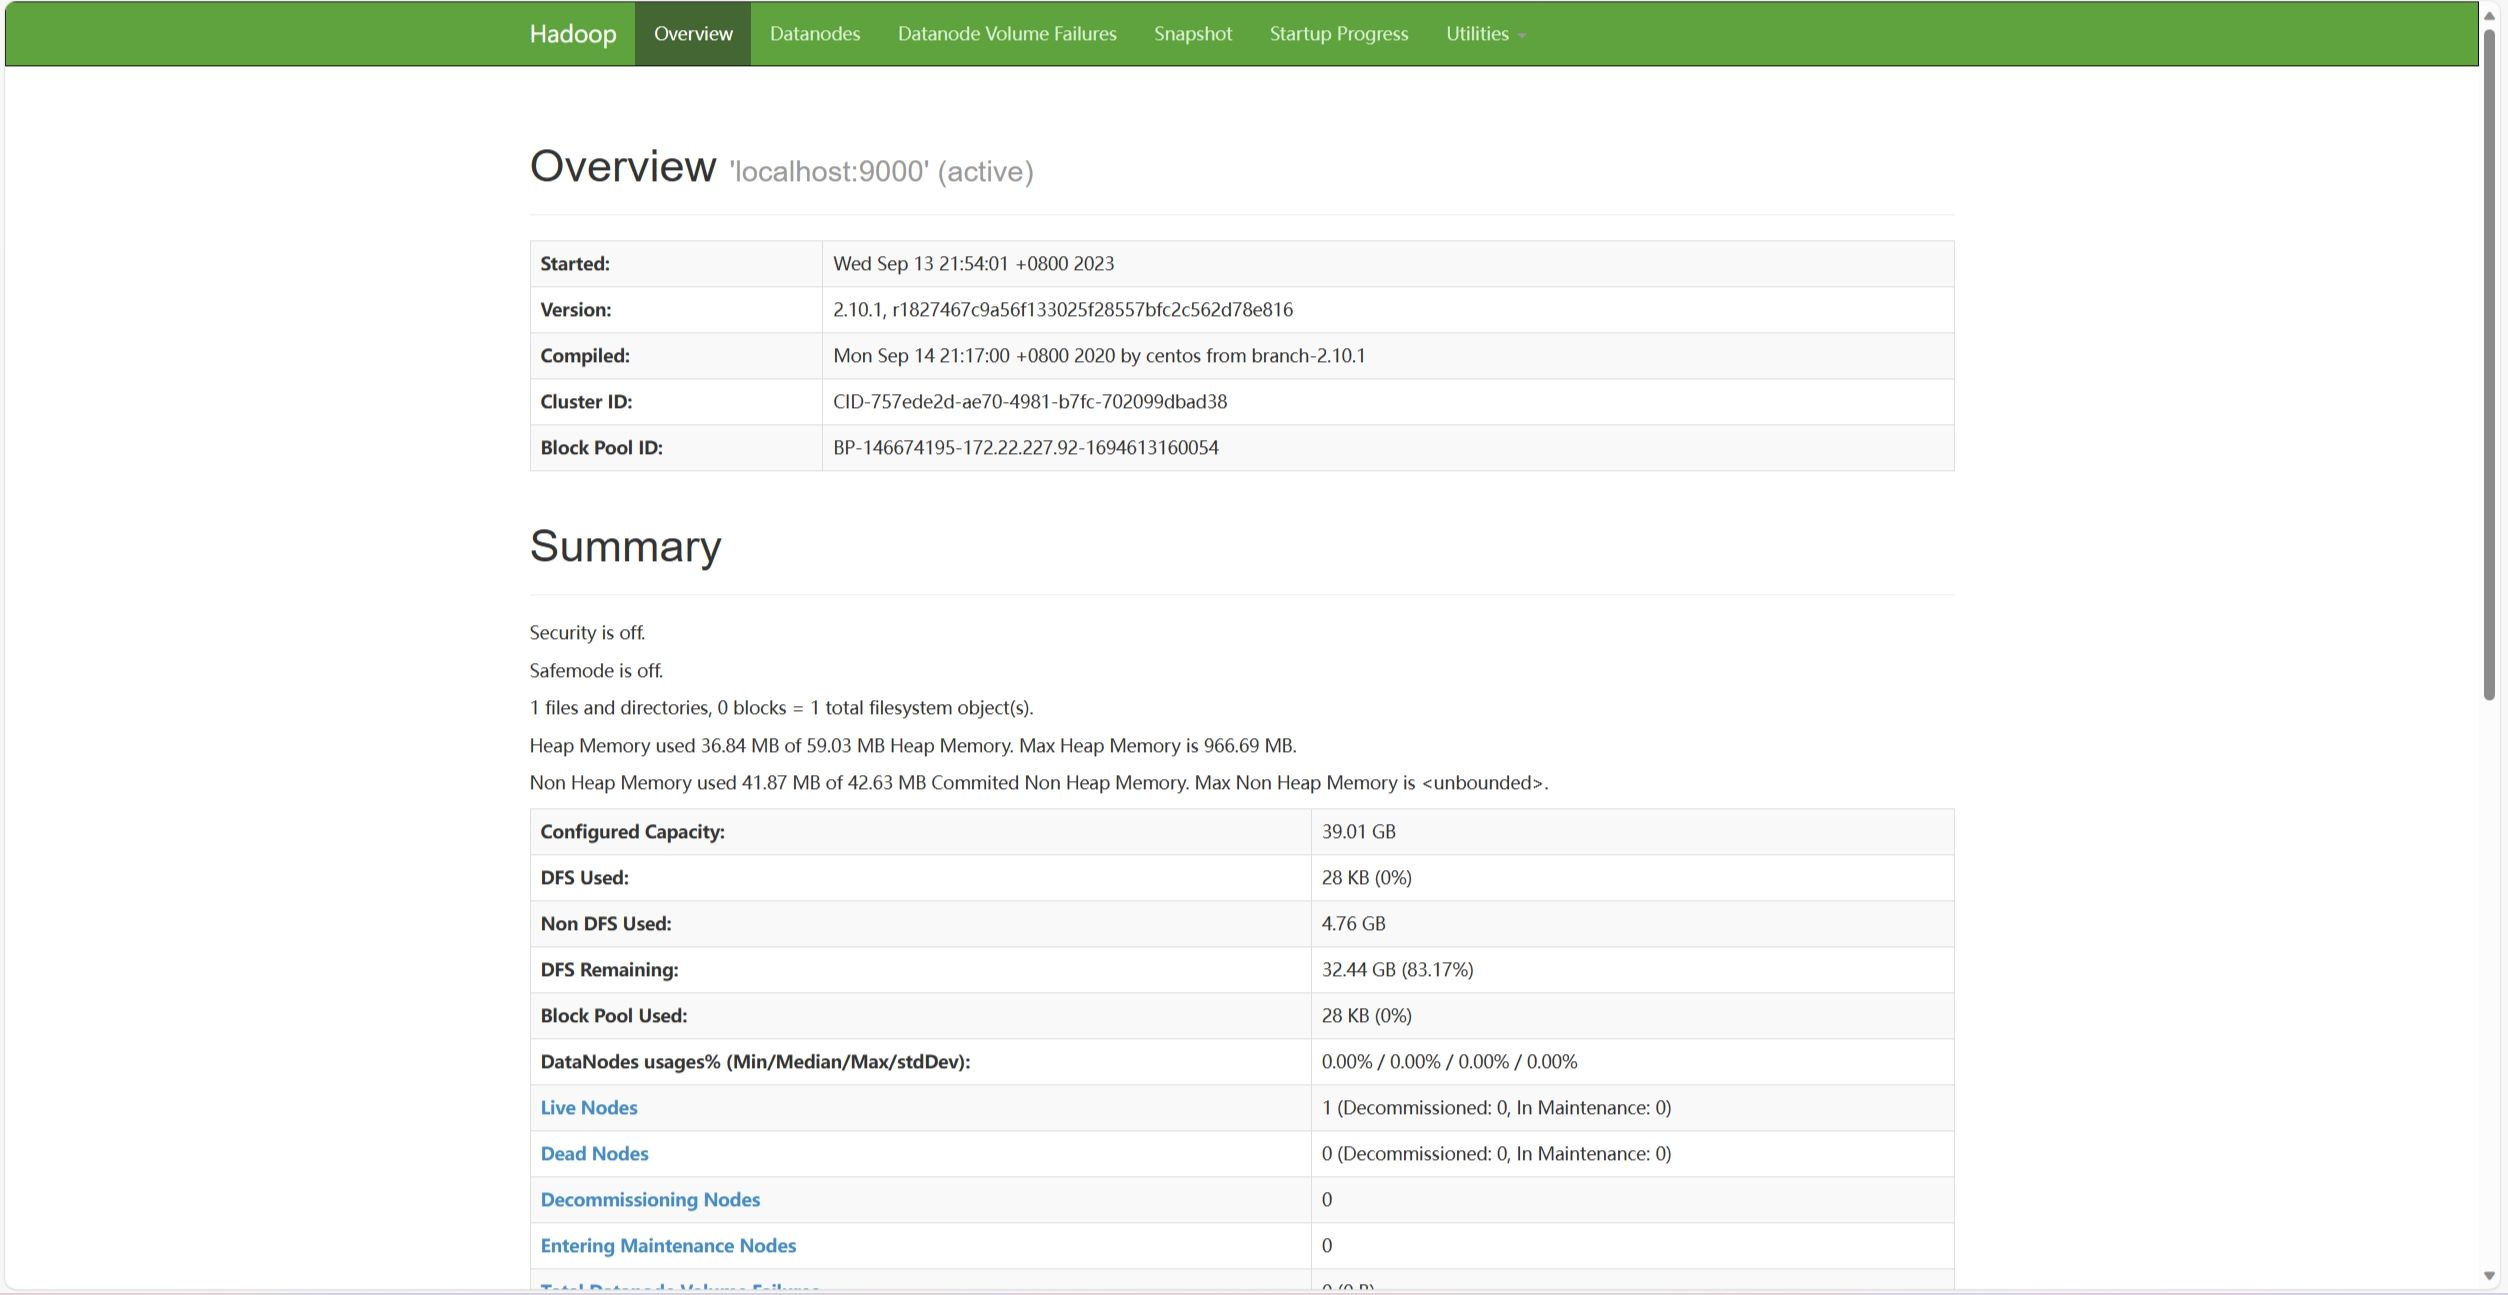
\includegraphics[width=0.7\textwidth]{./pic/12.jpg}
              \caption{50070端口}
          \end{figure}
\end{itemize}

\subsection*{1.4 安装scala}
通过\lstinline[language=bash]|apt install scala|安装Scala,安装完成后通过\lstinline[language=bash]|scala -version|查看Scala版本。
\begin{figure}[H]
    \centering
    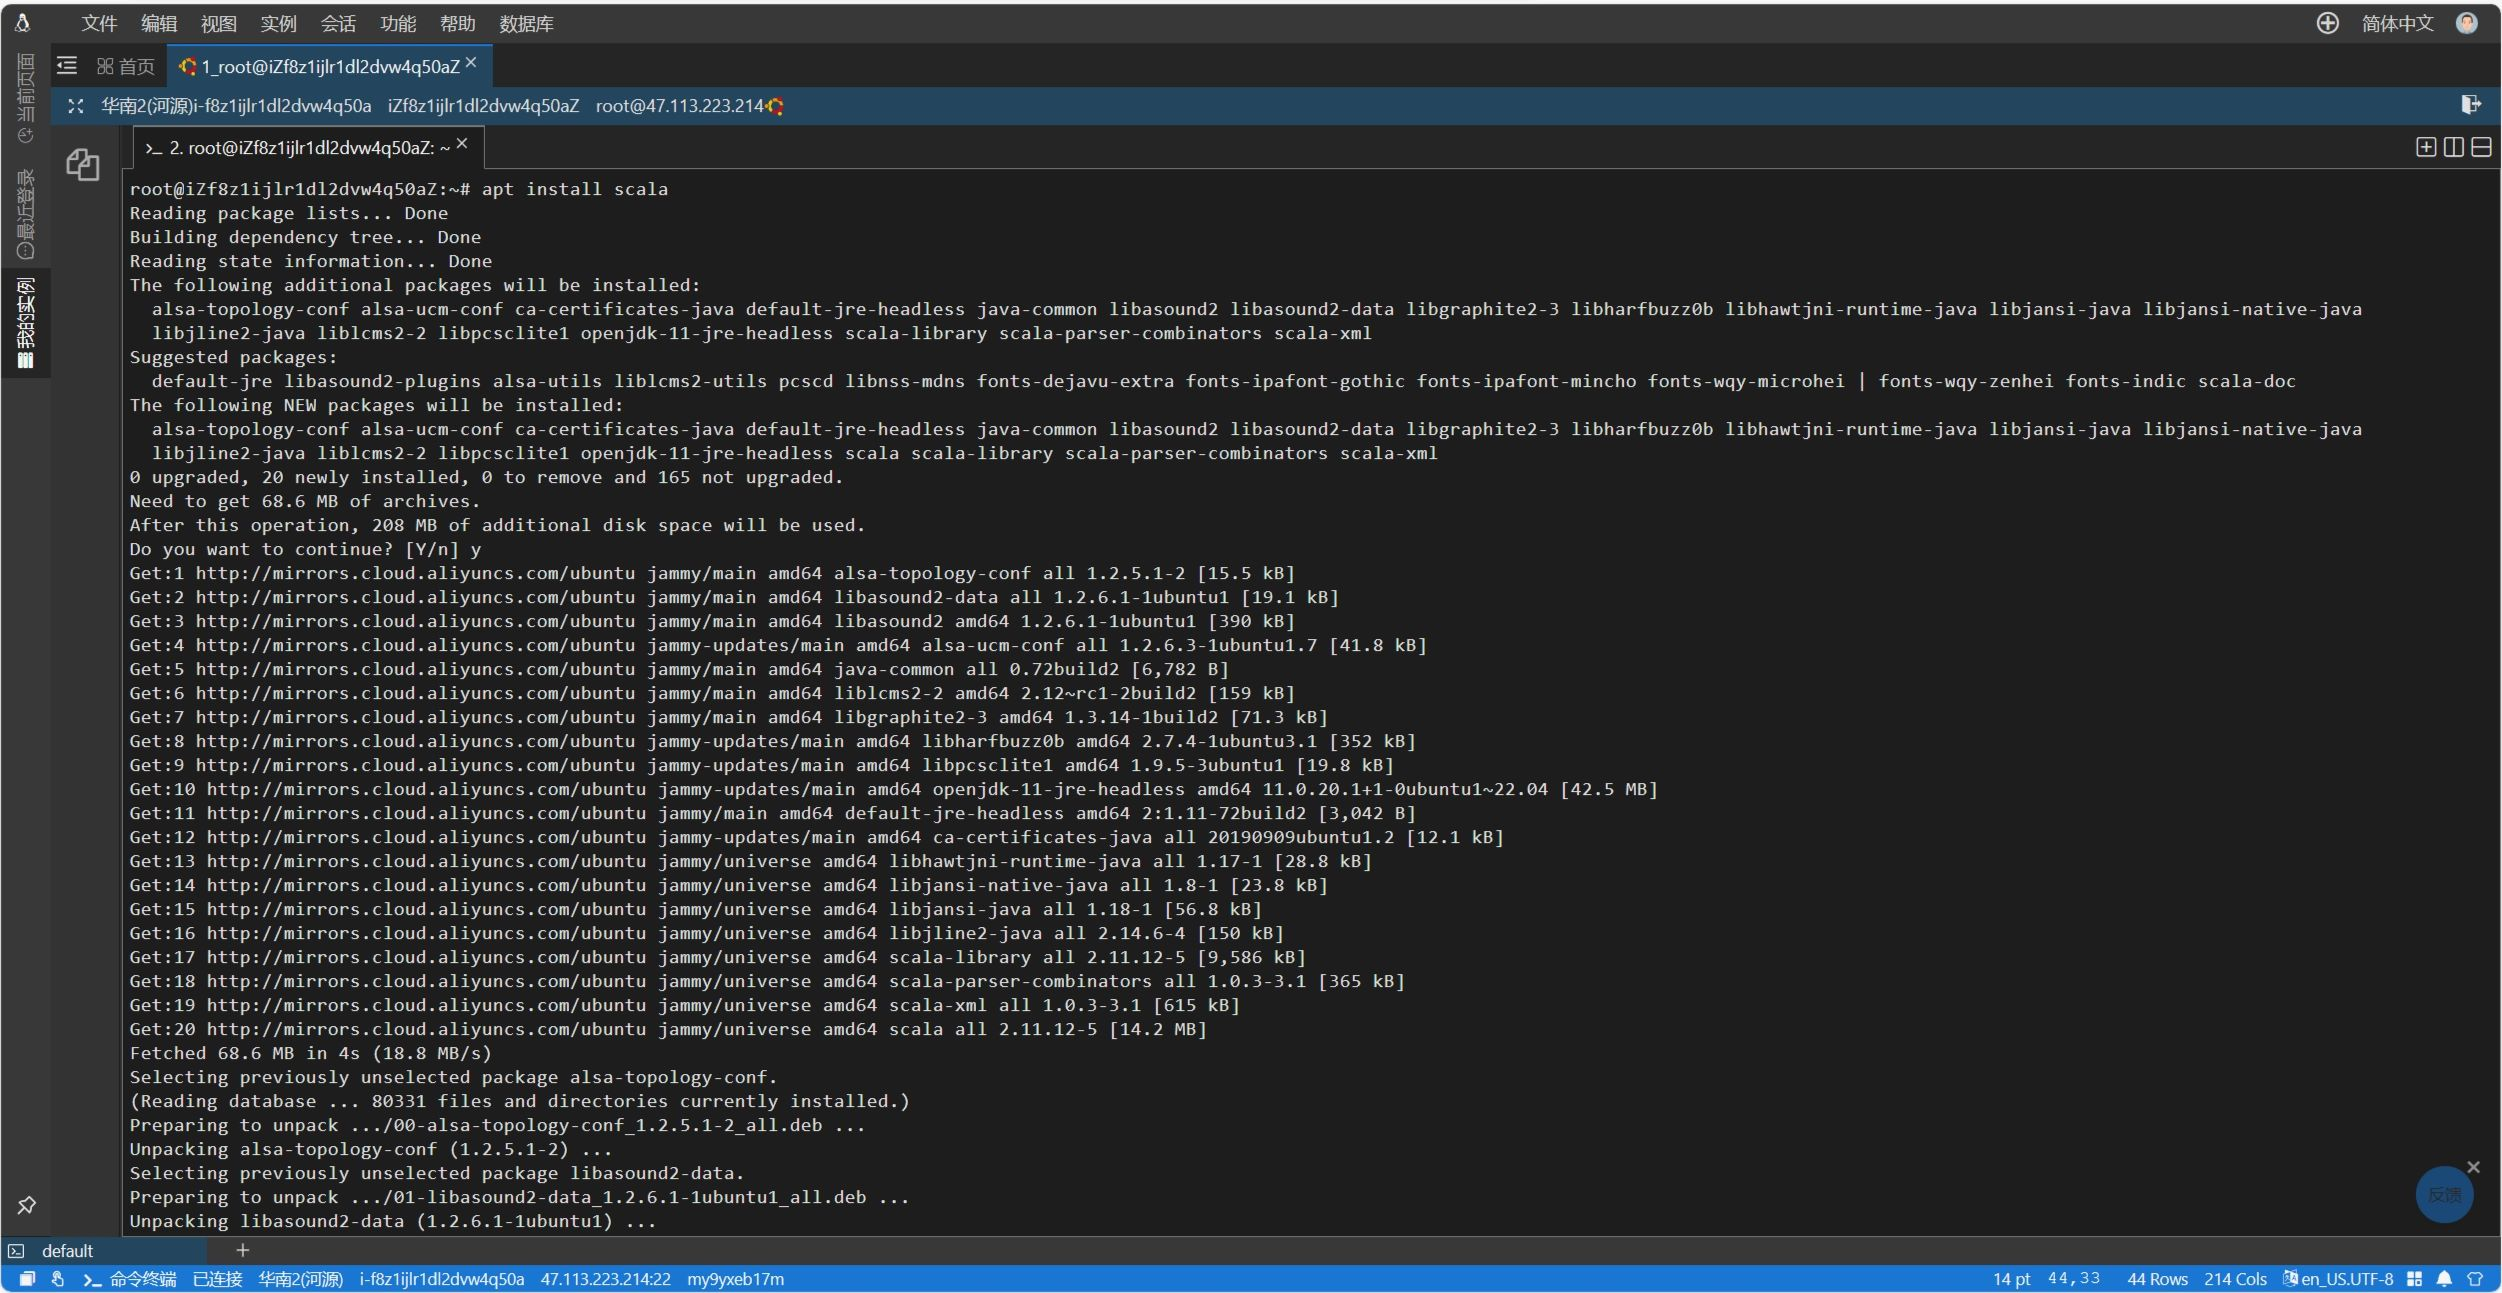
\includegraphics[width=0.7\textwidth]{./pic/13.jpg}
    \caption{安装Scala}
\end{figure}
\begin{figure}[H]
    \centering
    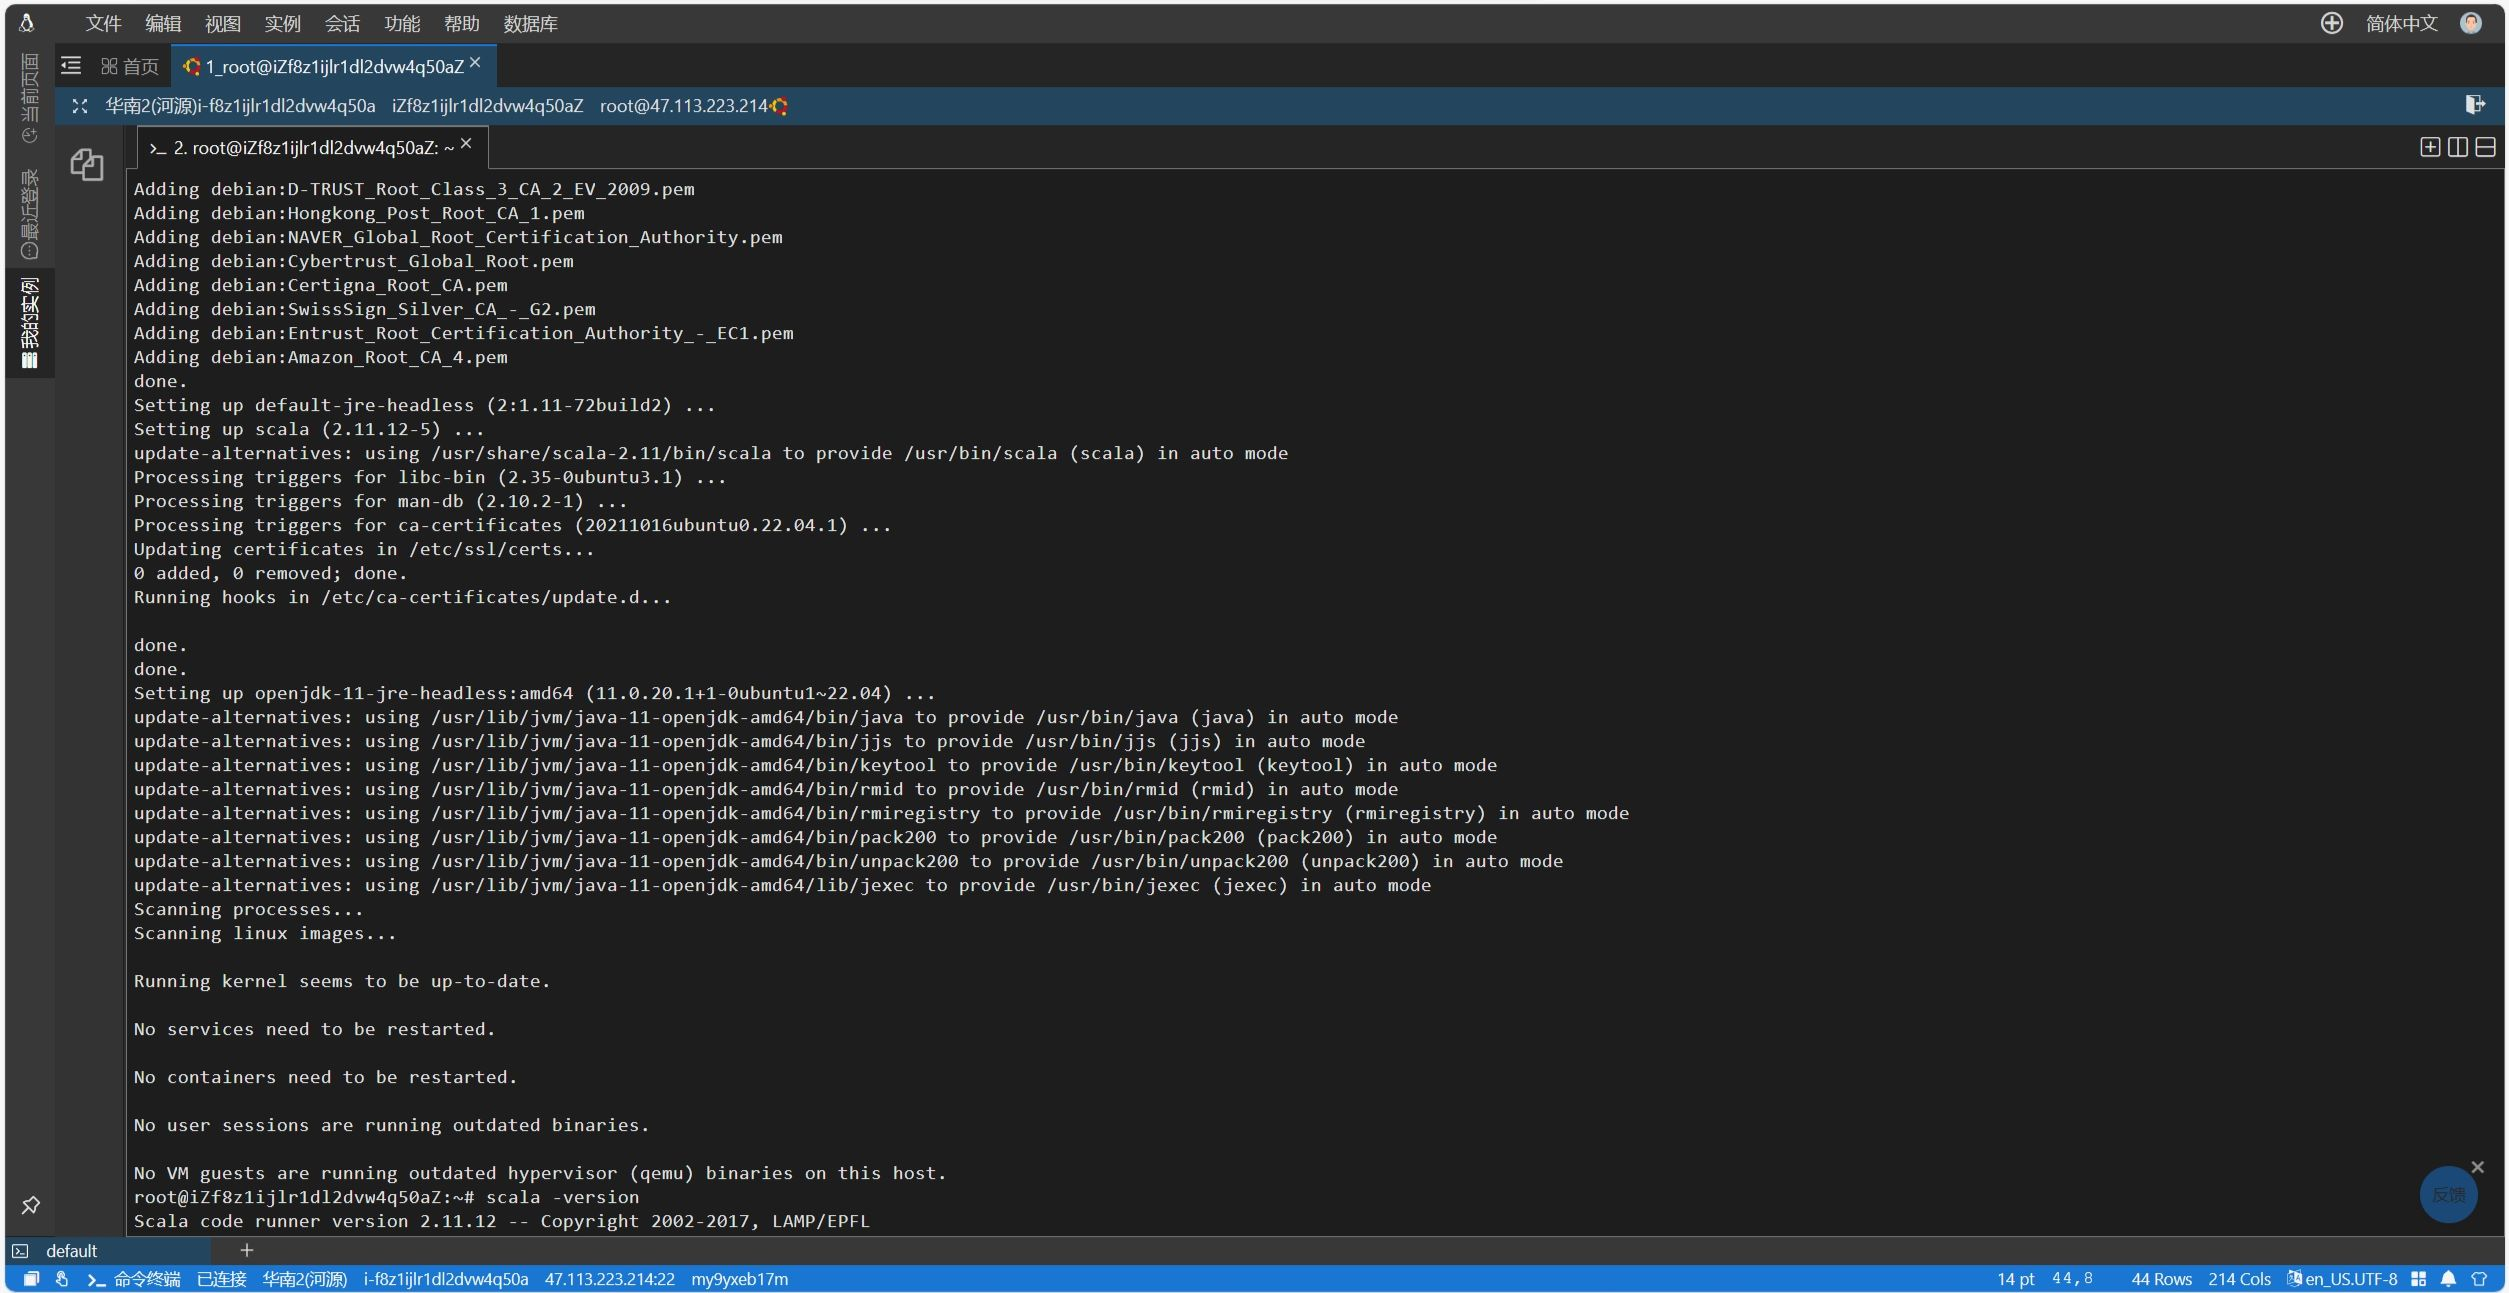
\includegraphics[width=0.7\textwidth]{./pic/14.jpg}
    \caption{查看Scala版本}
\end{figure}

\subsection*{1.5 安装spark}
\begin{itemize}
    \item 执行\lstinline[language=bash]|curl -O https://archive.apache.org/dist/spark/spark-3.2.4/spark-3.2.4-bin-hadoop2.7.tgz|下载spark压缩包并解压。
          \begin{figure}[H]
              \centering
              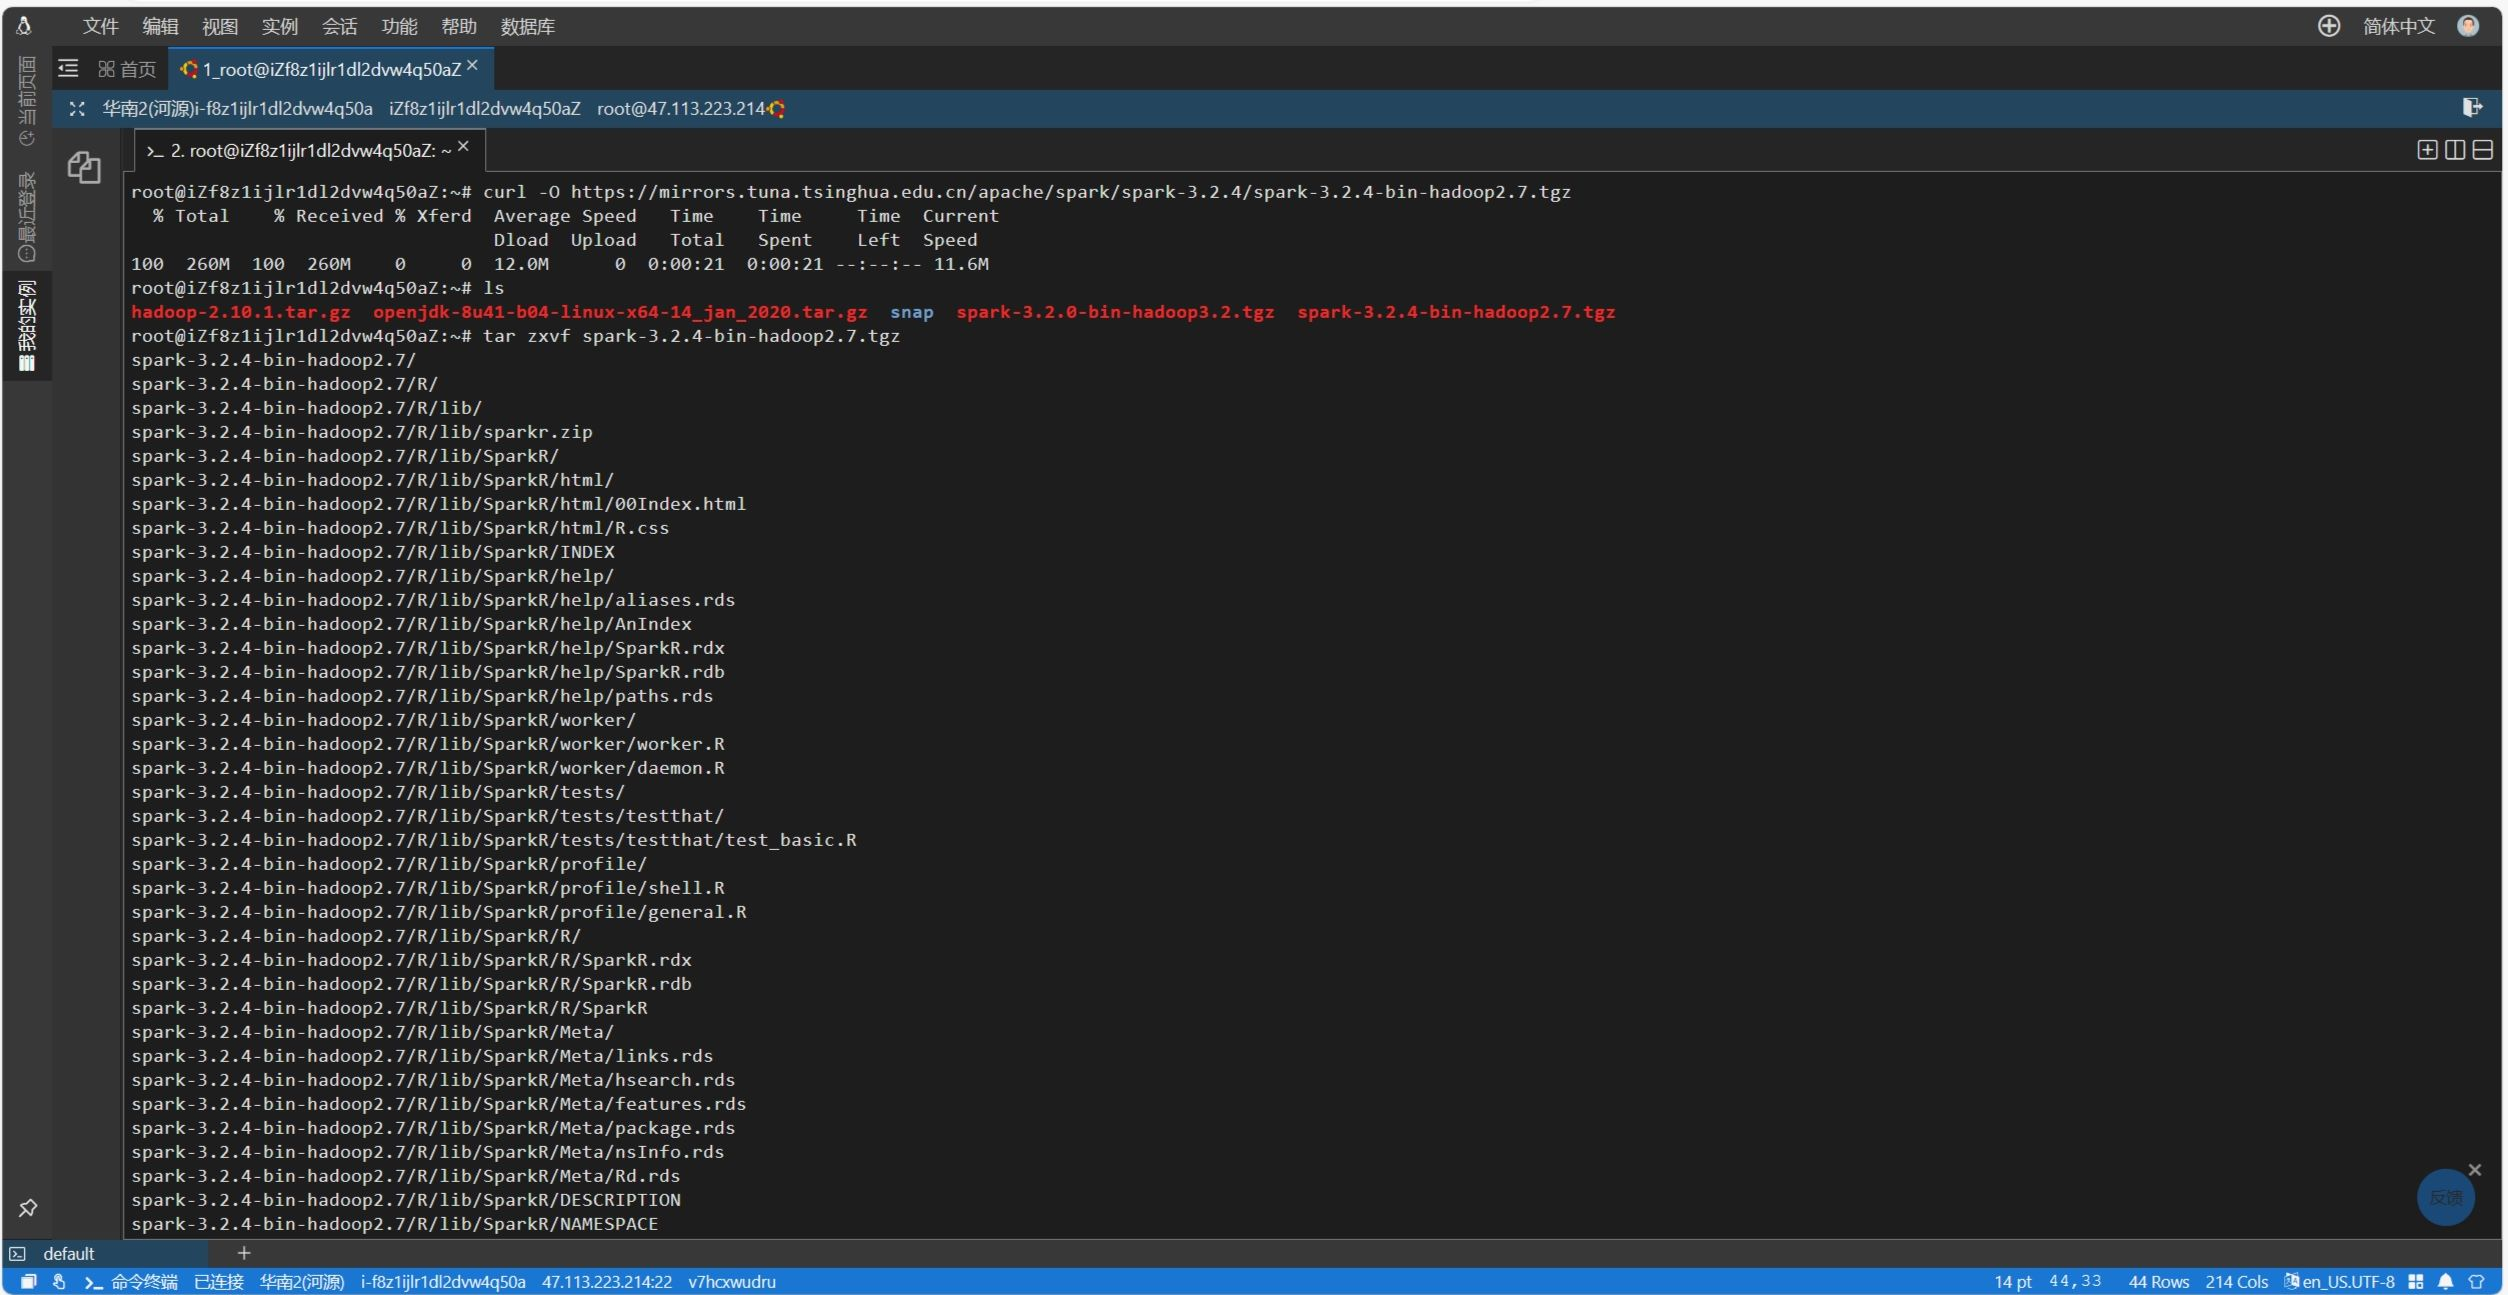
\includegraphics[width=0.7\textwidth]{./pic/15.jpg}
              \caption{下载spark并解压}
          \end{figure}
    \item 移动安装包并配置环境变量
          \begin{figure}[H]
              \centering
              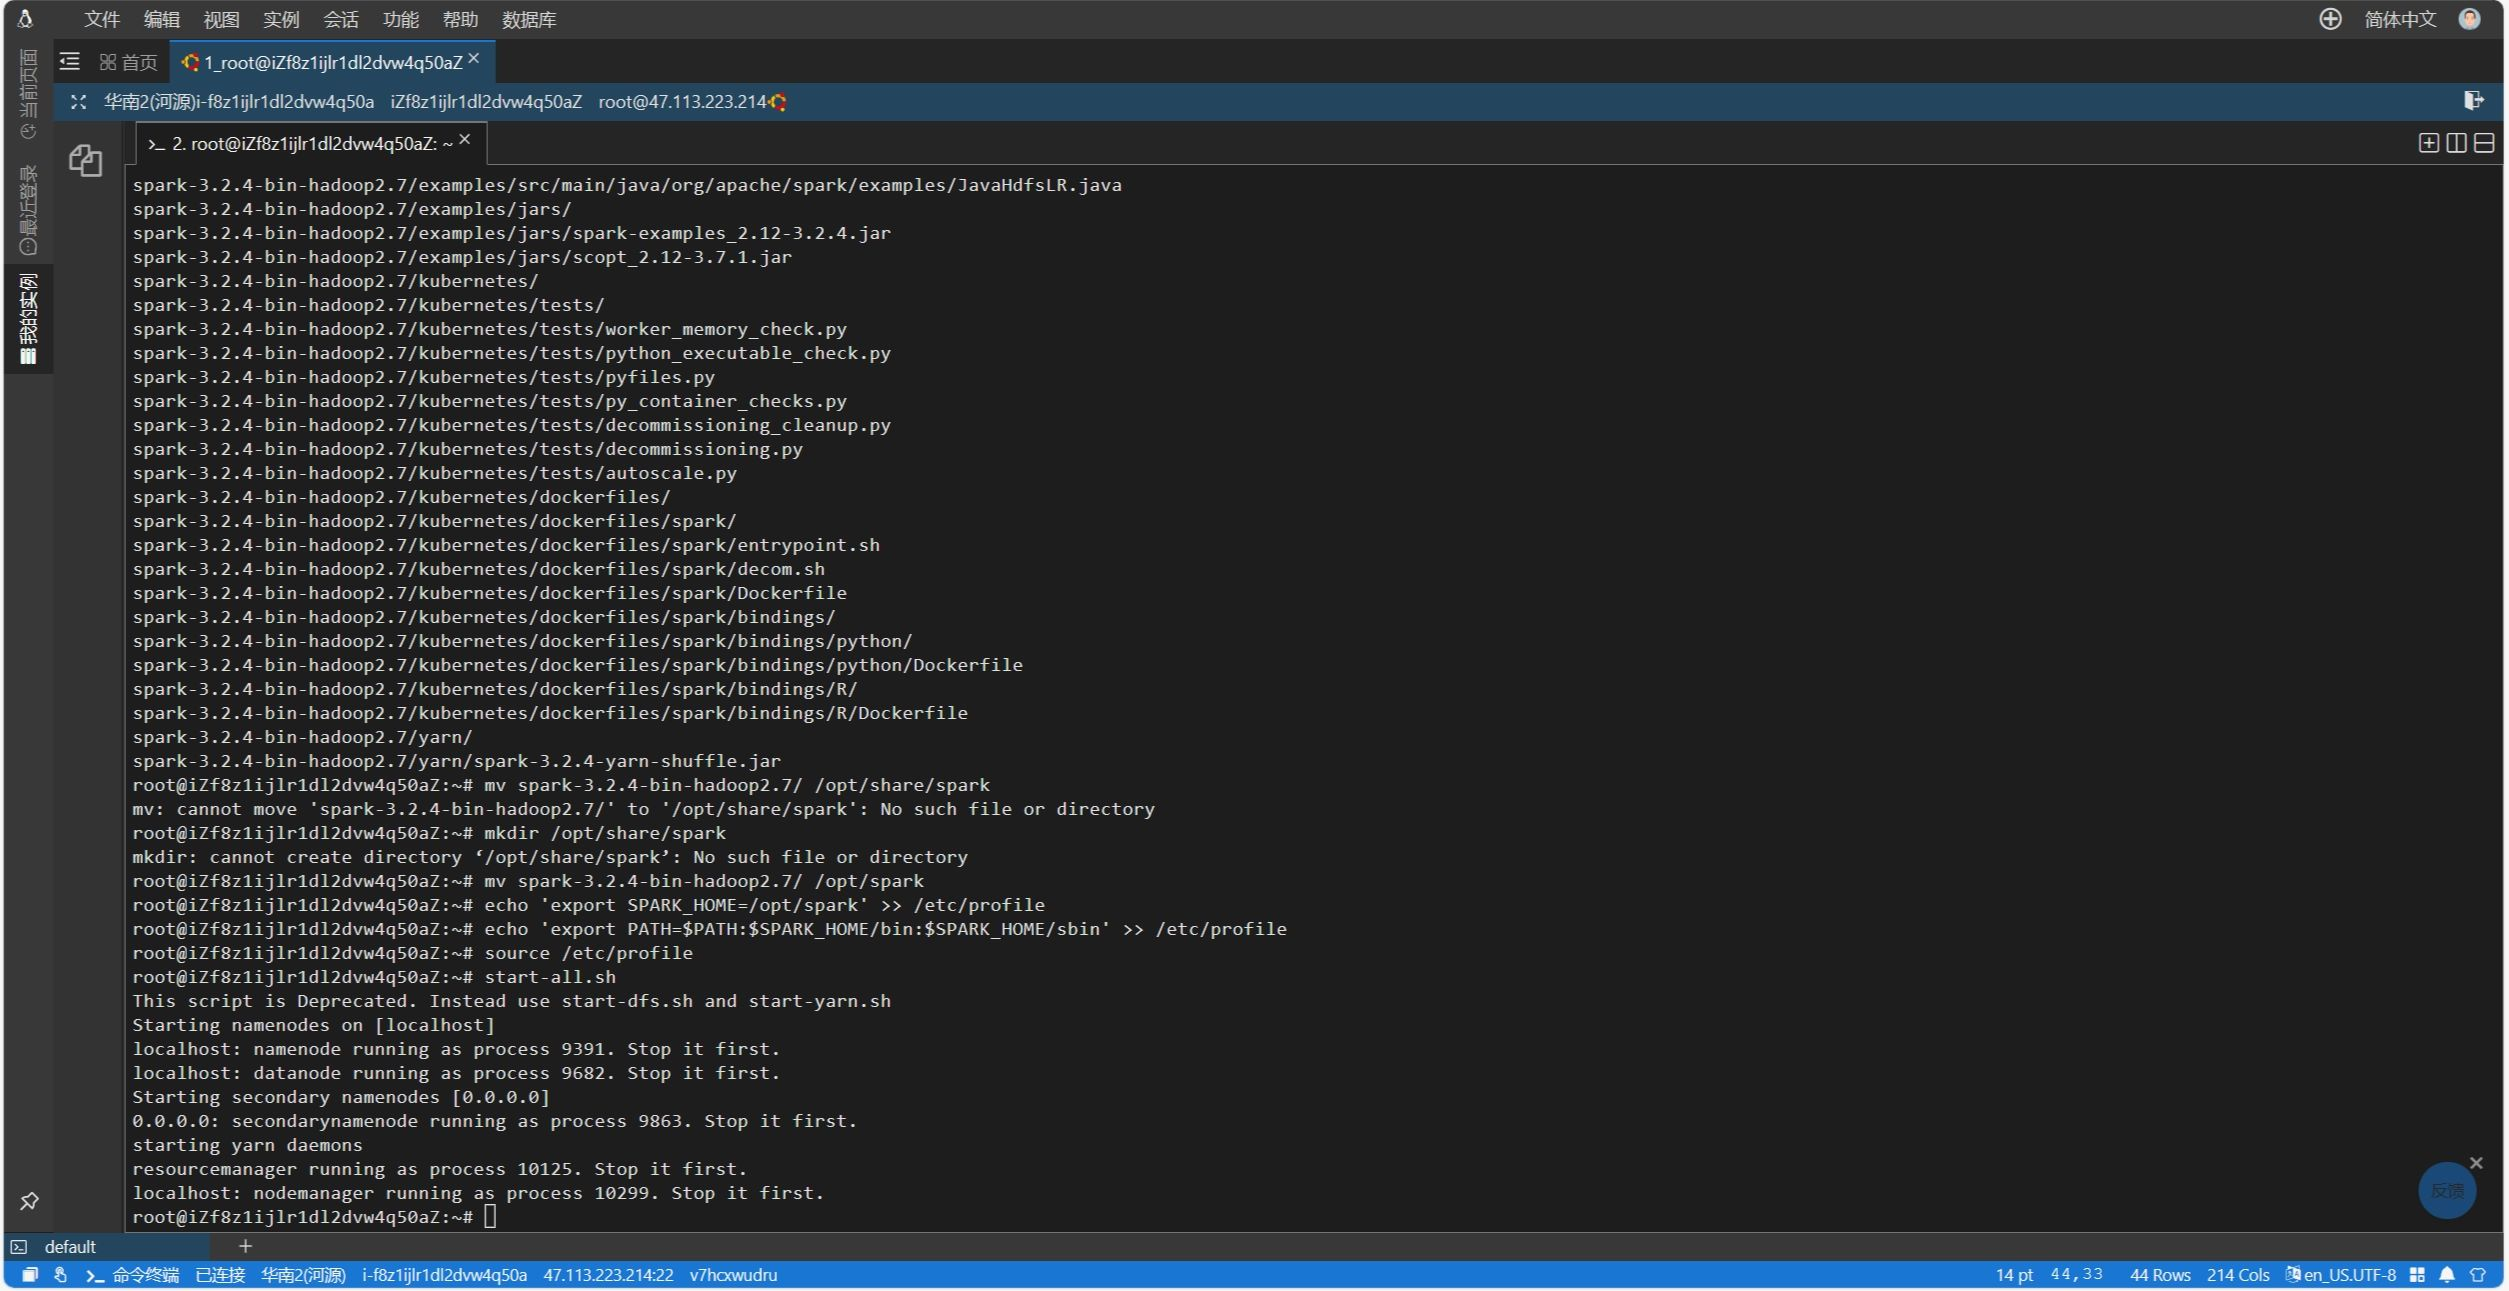
\includegraphics[width=0.7\textwidth]{./pic/16.jpg}
              \caption{配置spark}
          \end{figure}
    \item 启动spark-shell以验证安装
          \begin{figure}[H]
              \centering
              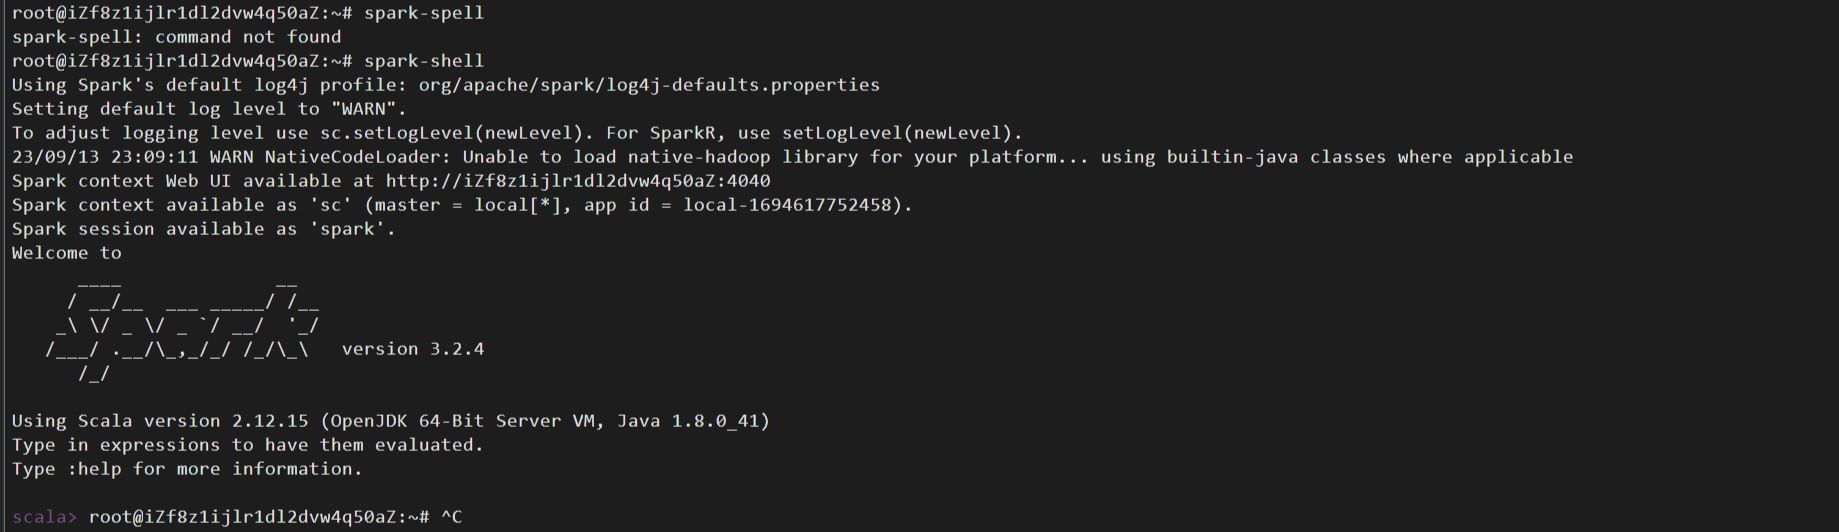
\includegraphics[width=0.7\textwidth]{./pic/17.jpg}
              \caption{spark-shell}
          \end{figure}
\end{itemize}

\subsection*{1.6 安装sbt}
通过执行如图命令安装sbt。
\begin{figure}[H]
    \centering
    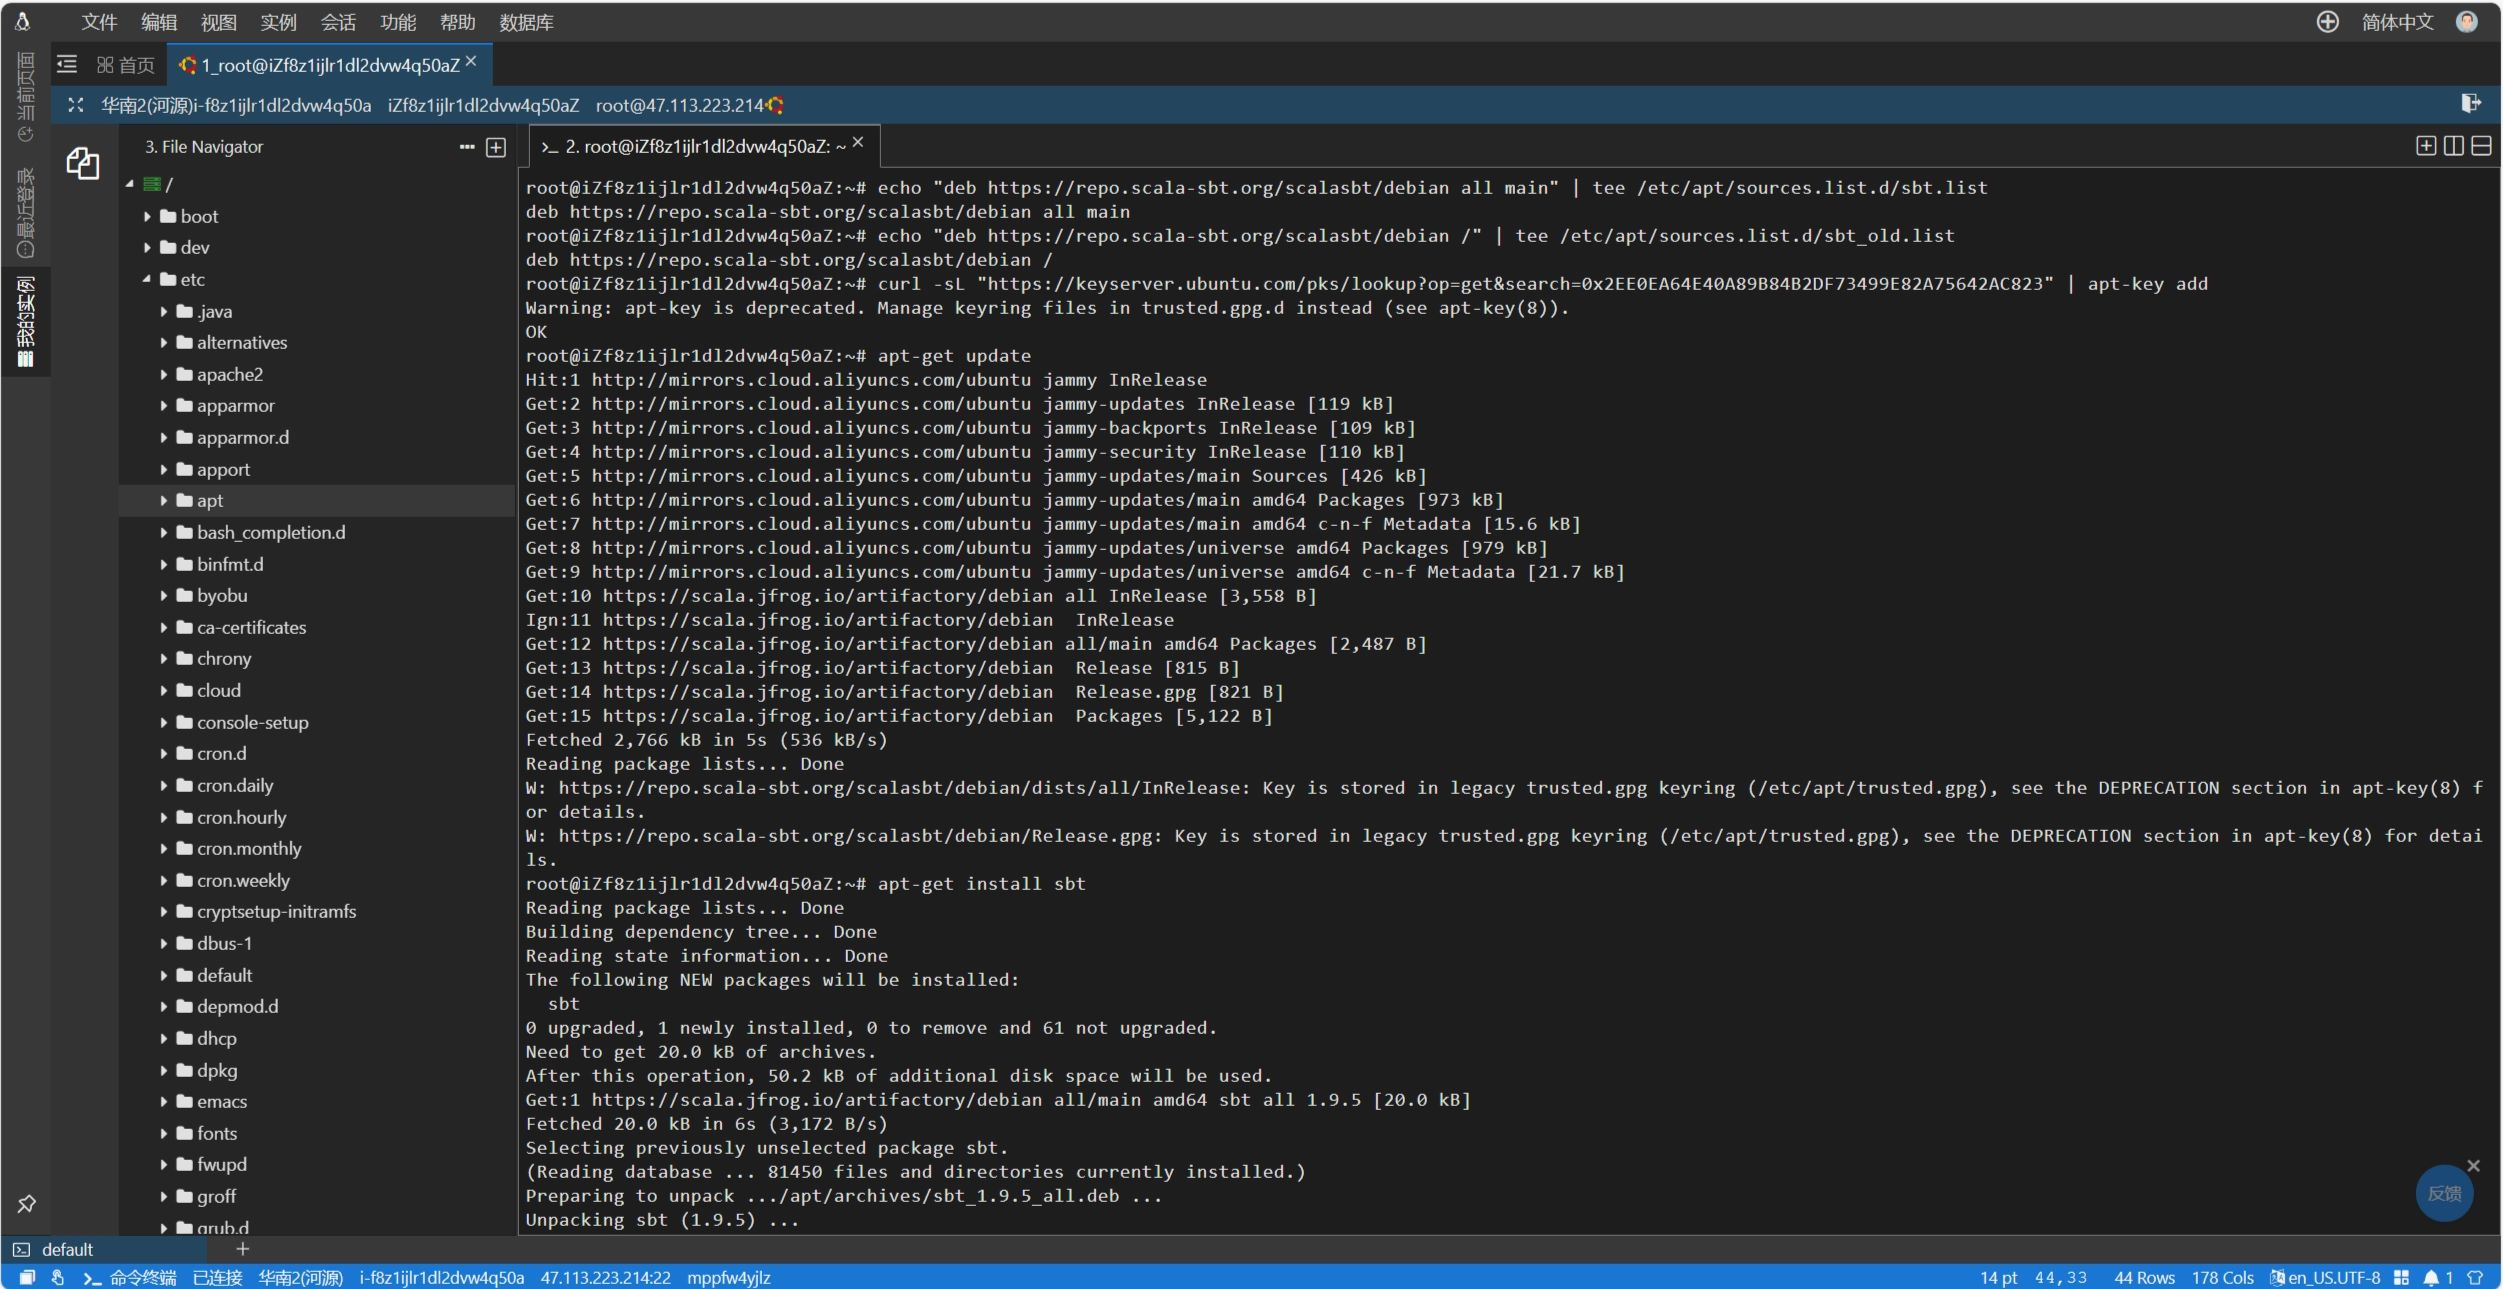
\includegraphics[width=0.7\textwidth]{./pic/21.jpg}
    \caption{安装sbt}
\end{figure}


\section{代码编写与运行}
\subsection*{2.1 编写代码}
\lstinputlisting[style=Style, caption=helloWorld, label=code:example]{../Hello.scala}
\lstinputlisting[style=Style, caption=wordCount, label=code:example]{../WordCount.scala}

\subsection*{2.2 编译运行helloWorld代码}
通过scalac命令编译之后使用scala命令运行
\begin{figure}[H]
    \centering
    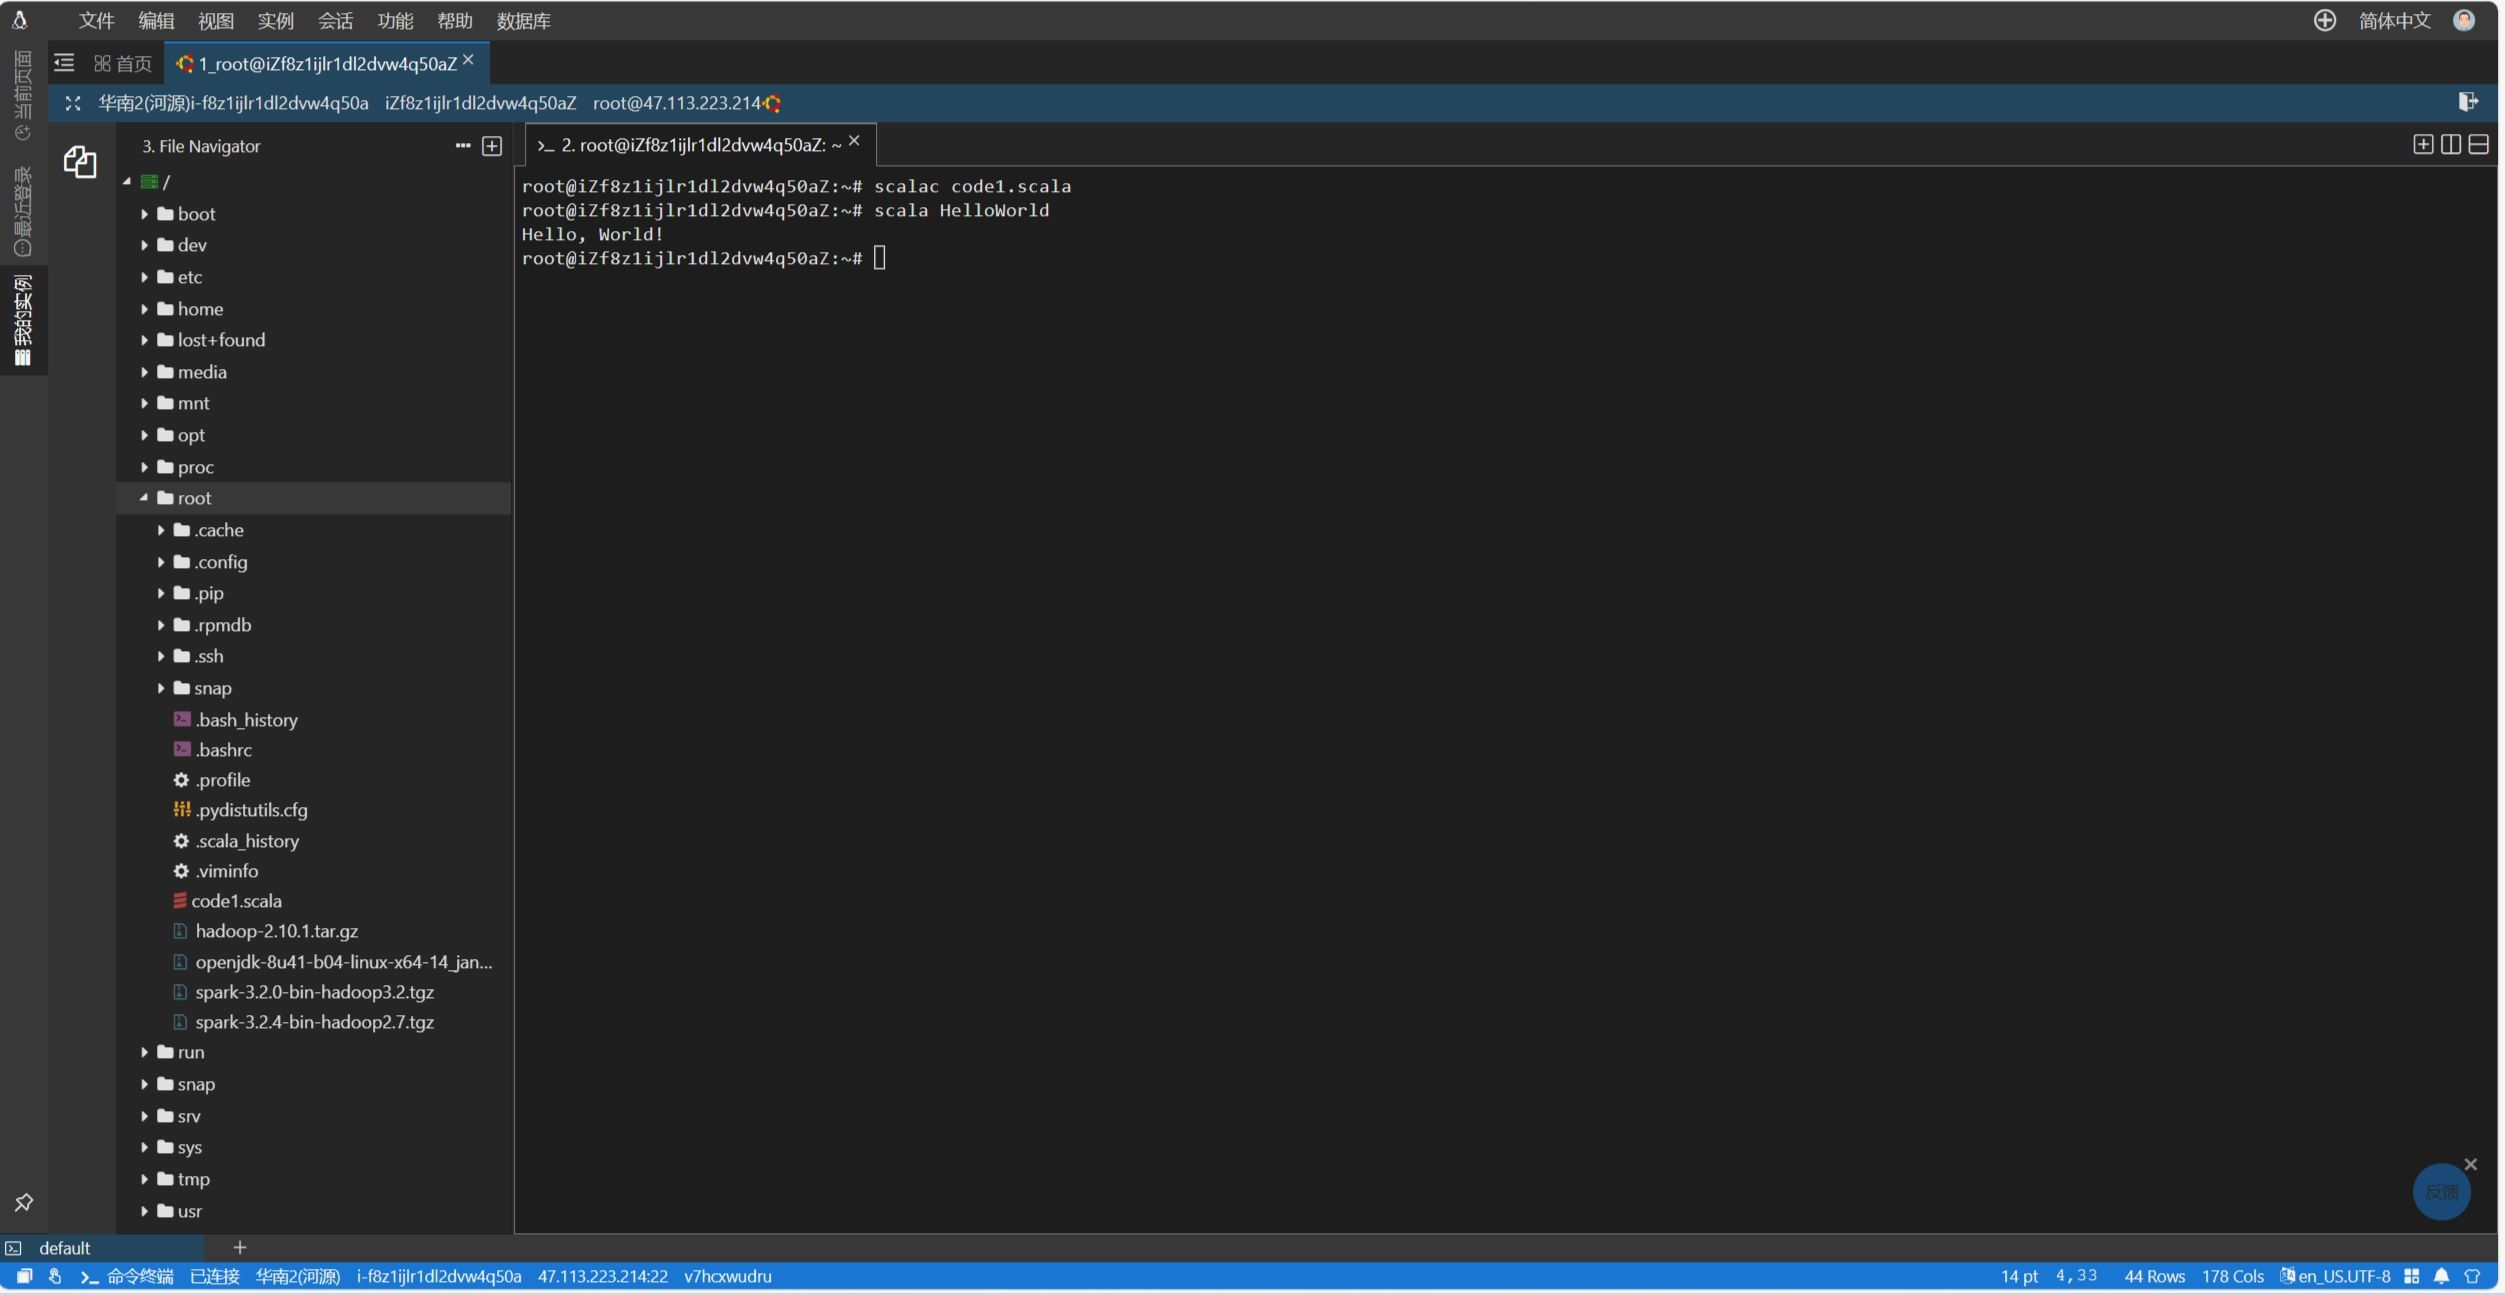
\includegraphics[width=0.7\textwidth]{./pic/19.jpg}
    \caption{运行helloWorld}
\end{figure}

\subsection*{2.2 打包运行wordCount代码}
\begin{itemize}
    \item 使用\lstinline[language=bash]|sbt package|打包wordCount项目
    \begin{figure}[H]
        \centering
        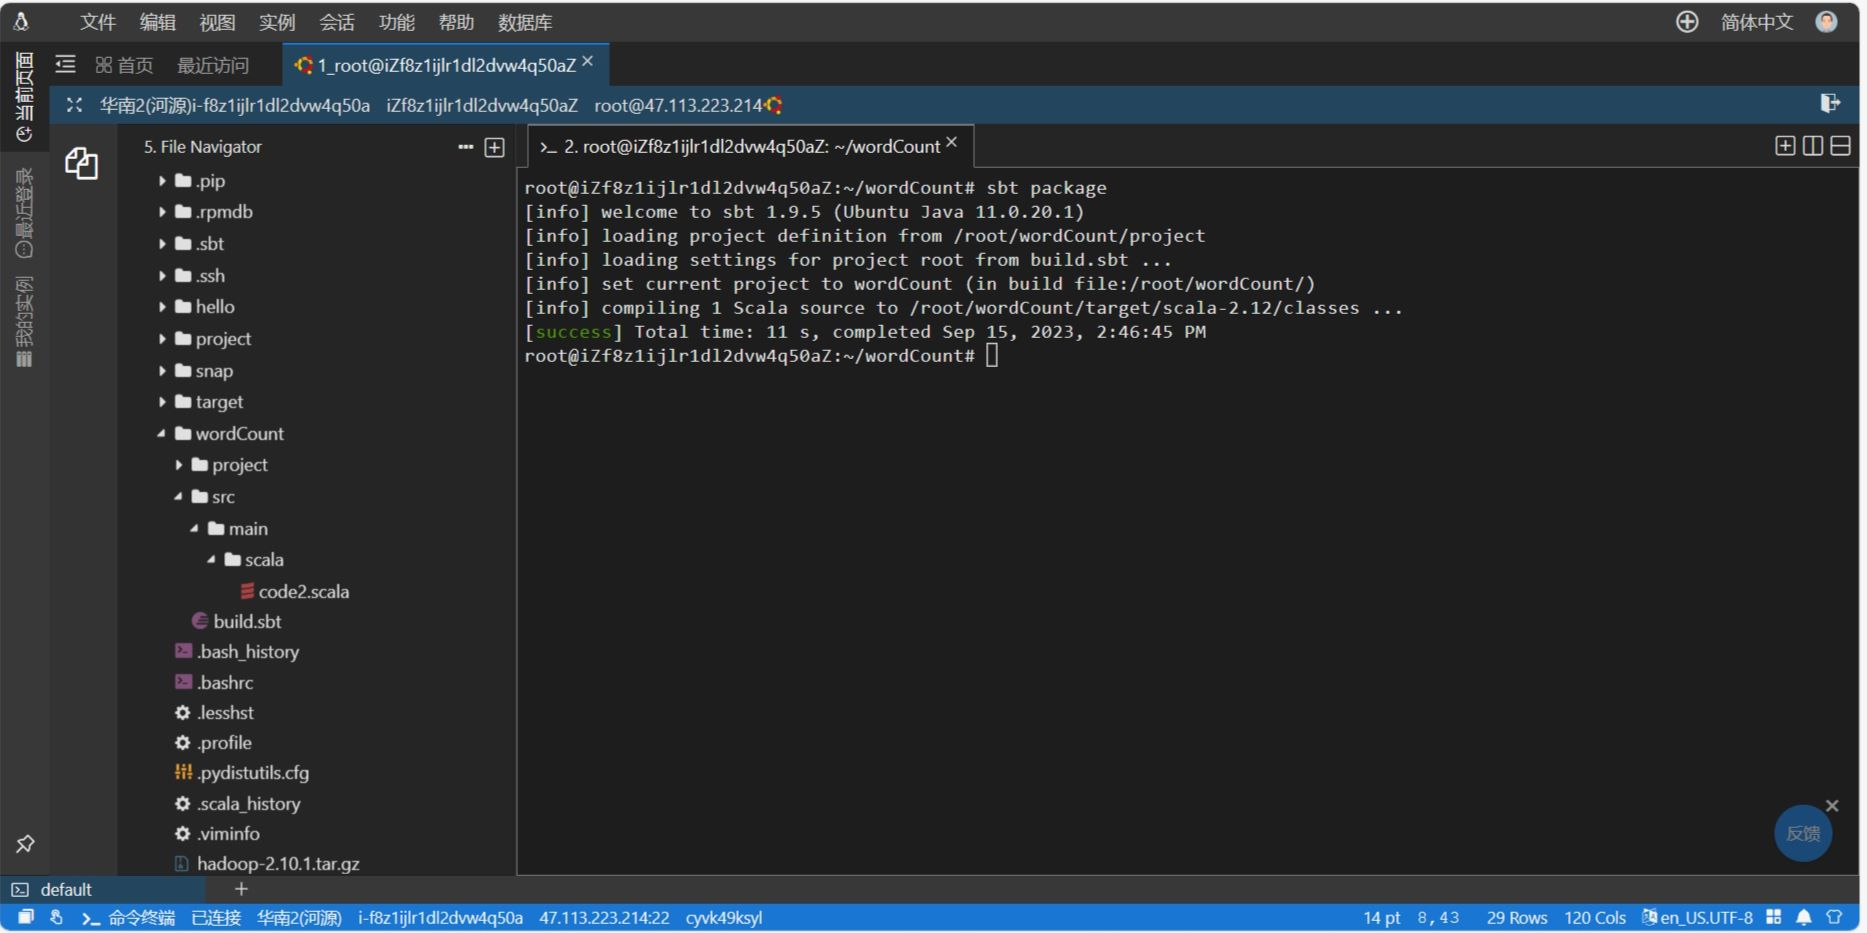
\includegraphics[width=0.7\textwidth]{./pic/24.jpg}
        \caption{sbt打包}
    \end{figure}
    \item 通过\lstinline[language=bash]|start-all.sh|启动Hadoop并将test.txt文件上传到hdfs。在Web界面查看。
    \begin{figure}[H]
        \centering
        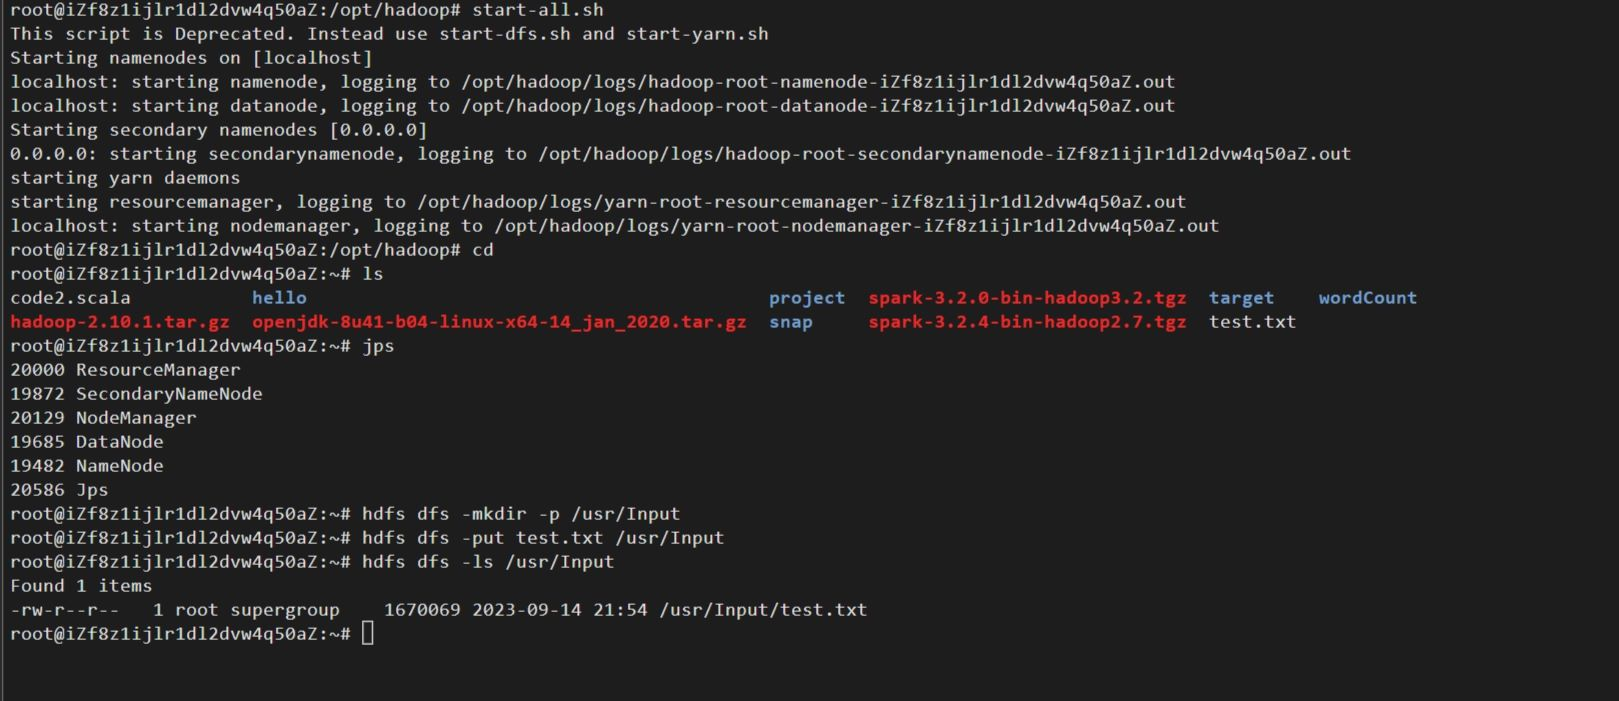
\includegraphics[width=0.7\textwidth]{./pic/22.jpg}
        \caption{上传文件}
    \end{figure}
    \begin{figure}[H]
        \centering
        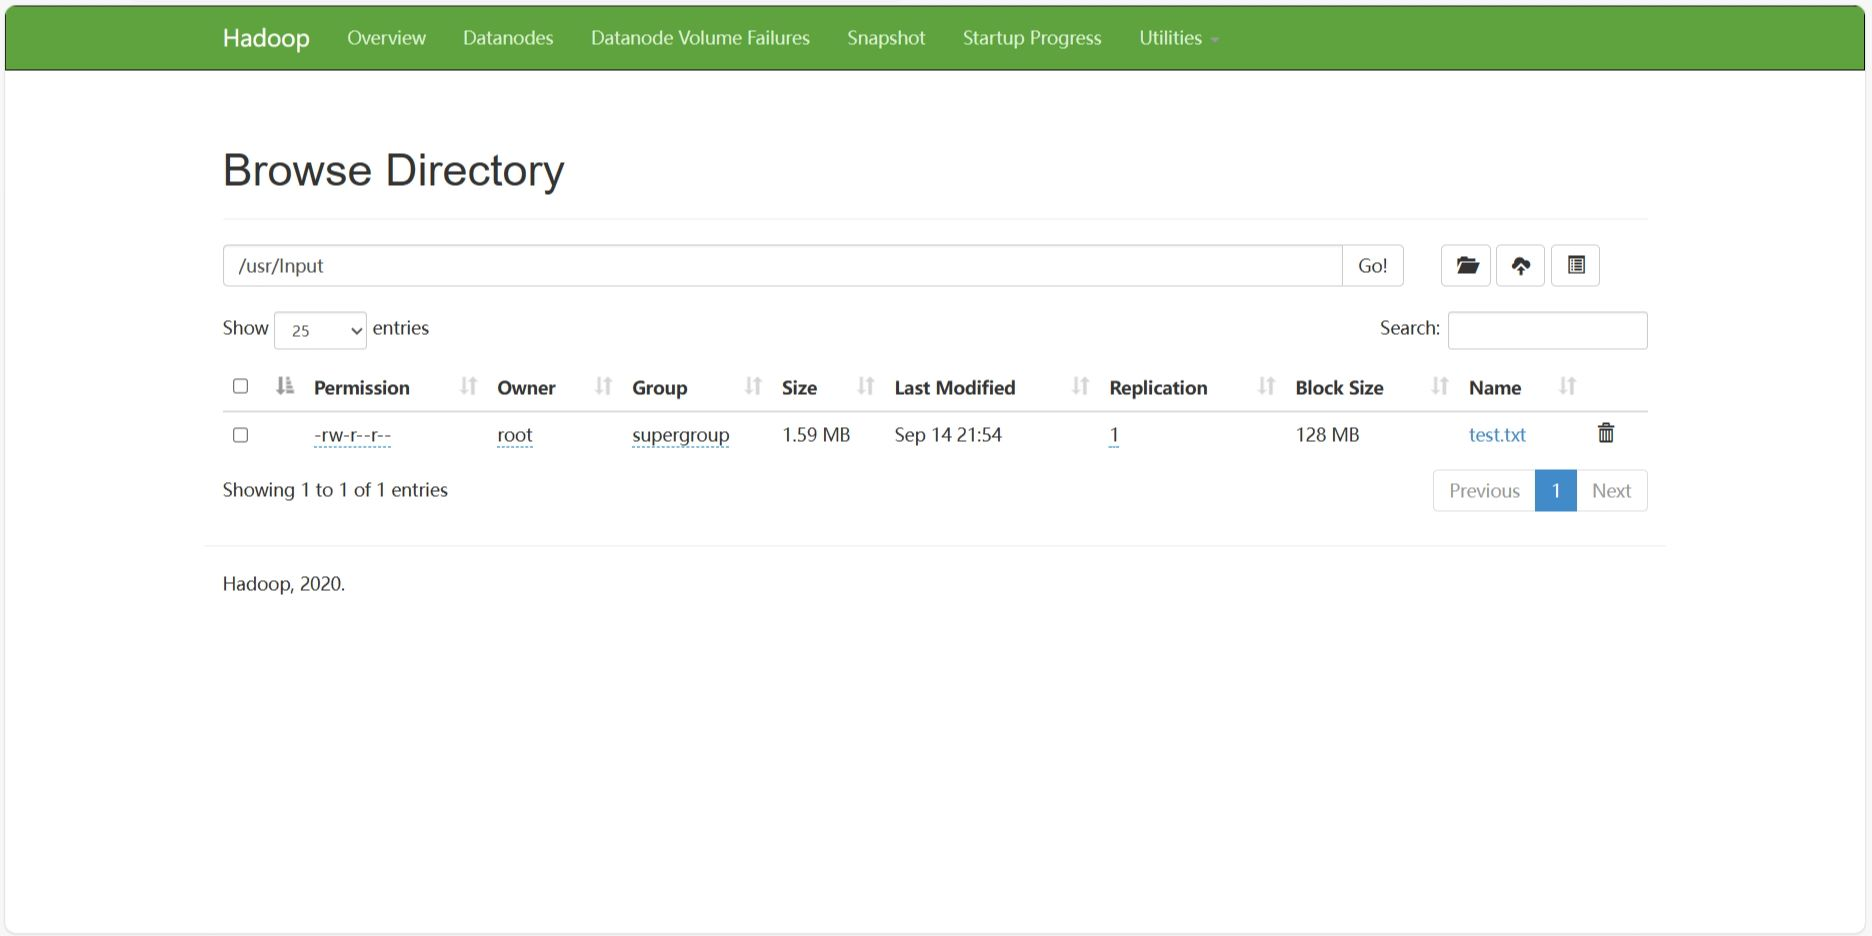
\includegraphics[width=0.7\textwidth]{./pic/23.jpg}
        \caption{Hadoop Web}
    \end{figure}
    \item 将打包好的jar包通过spark-submit提交运行。图24是运行结果(部分)。经过核实,程序运行正常。
    \begin{figure}[H]
        \centering
        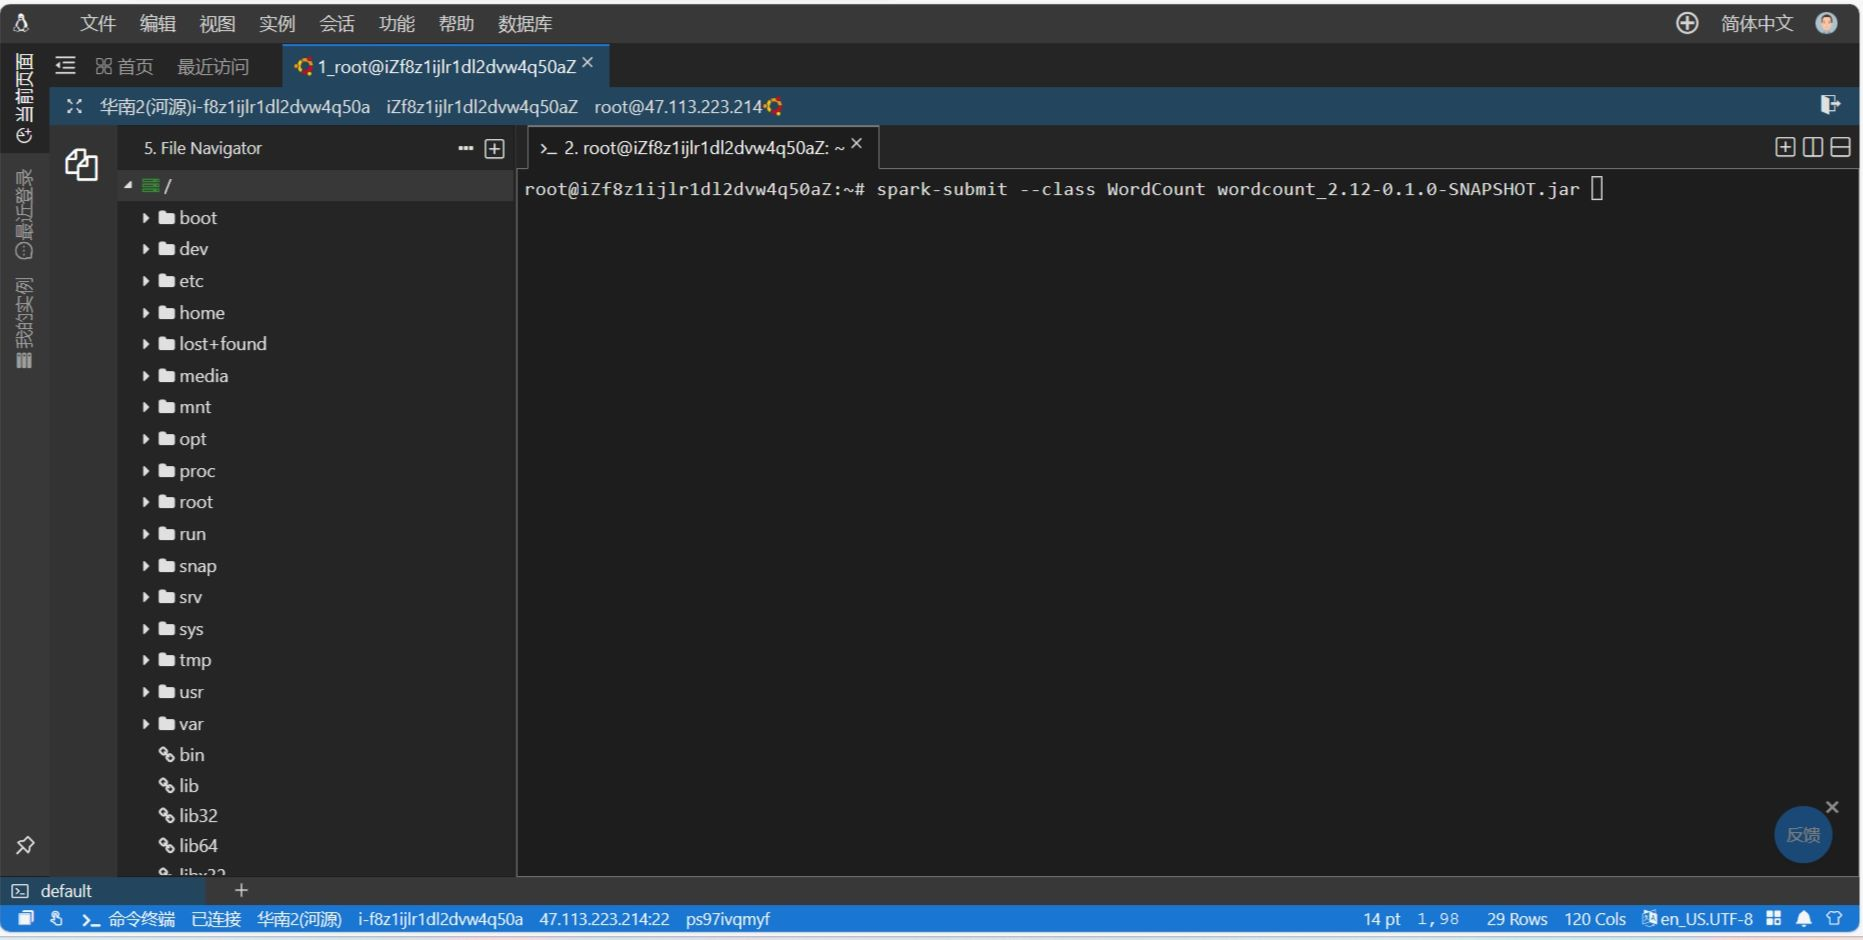
\includegraphics[width=0.7\textwidth]{./pic/26.jpg}
        \caption{spark-submit}
    \end{figure}
    \begin{figure}[H]
        \centering
        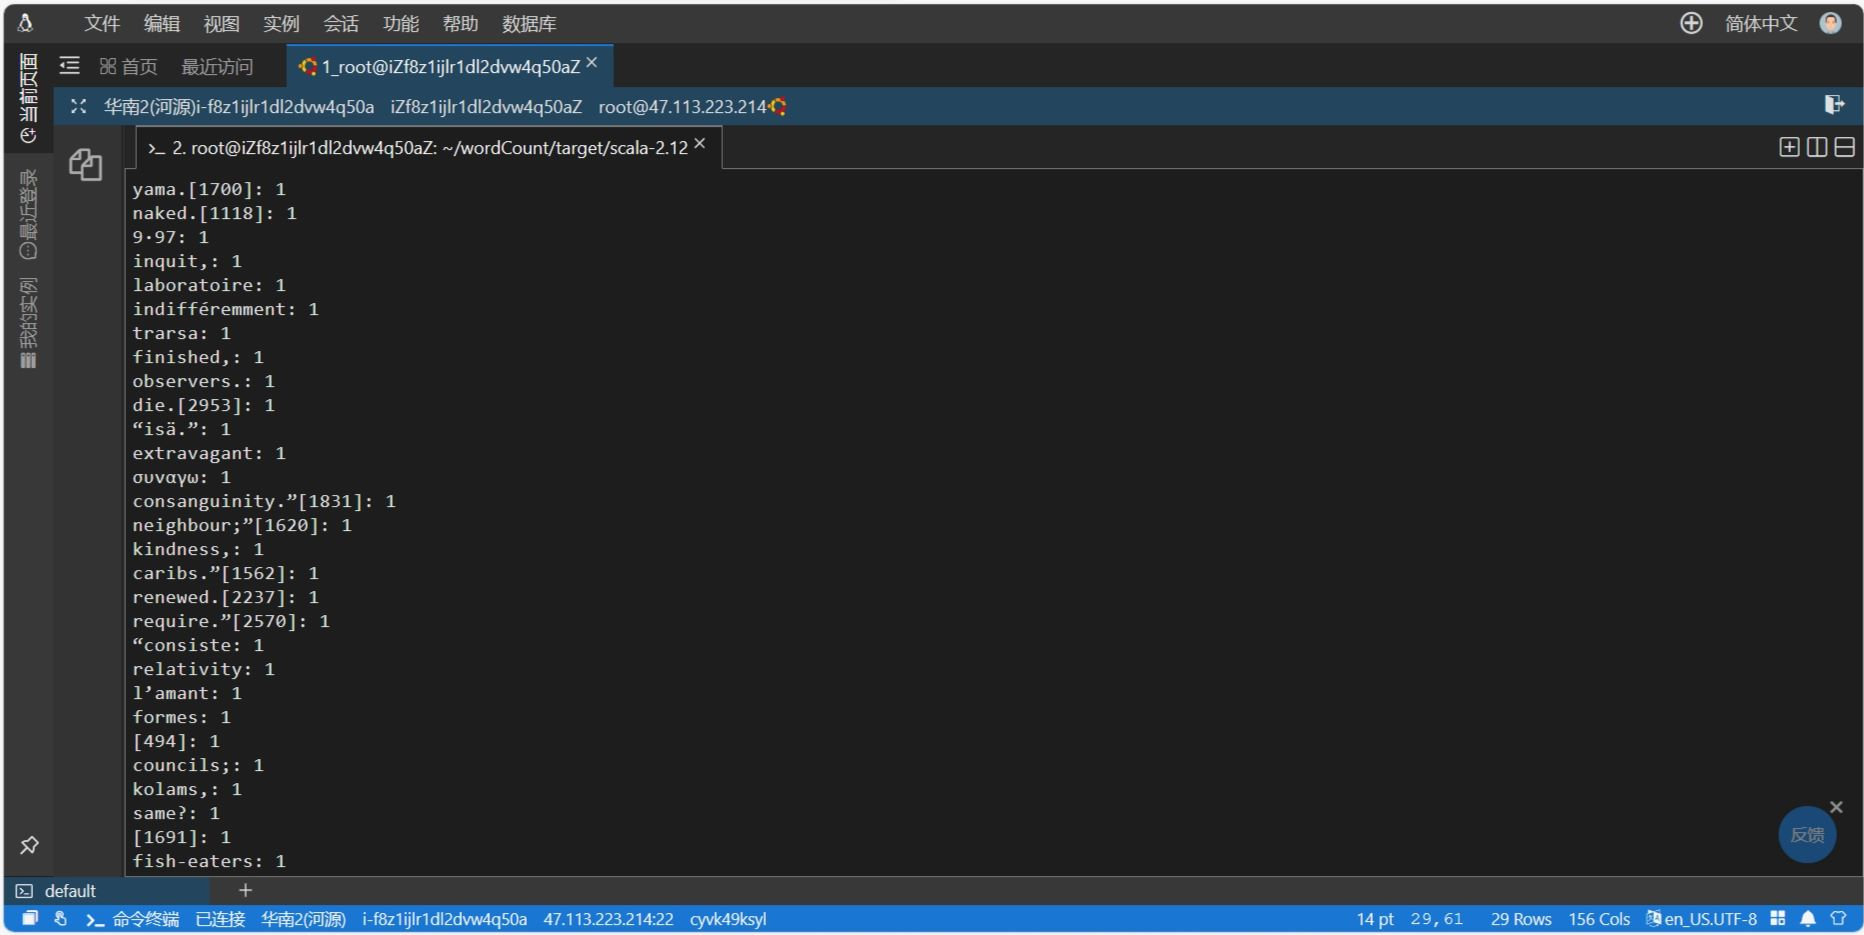
\includegraphics[width=0.7\textwidth]{./pic/25.jpg}
        \caption{运行结果}
    \end{figure}
    \item 通过\lstinline[language=bash]|stop-all.sh|关闭Hadoop
\end{itemize}


\section{挑战和克服方法}
\subsection*{3.1 寻找提供商}
起初并没有找到合适的平台服务提供商,在不断尝试和探索后,使用阿里云的学生ECS服务器
\subsection*{3.2 在服务器上将scala项目打包}
安装sbt的过程中遇到不少困难,期间服务器无法远程连接,只能重启。
由于项目结构错误,导致jar包无法在spark上运行,最终修改项目结构后,可以正常运行。
\end{document}